\begin{savequote}
``You cannot step in the same river twice''
\qauthor{Heracleitus, quoted in Plato, Cratylus, 402a}
\end{savequote}


\chapter{Jet Recollimation and Acceleration in an Evacuated Cavity} 
\label{JetRecollimationandAccelerationinanEvacuatedCavity}
%\minitoc

In this Chapter, we present simulations of jet propagation through an
ambient medium which we have envisioned as being evacuated by a previously
propagating jet or is a natural cavity in an inhomogeneous molecular cloud.
We show the collimative and accelerative
effects on the jet and compare with the standard case of a uniform
density medium propagation.  We have investigated the effects of ambient
material on the collimation and internal structure (specifically shocks)
of the jet.
We explore a parameter space of the jet-to-ambient
density ratio and the size of the density decrement
in the cavity, as well as the inclusion of (atomic) radiative cooling.
We demonstrate that the presence of a cavity can strongly recollimate the jet -
although this effect is lessened if radiative cooling is present.
The cavity also strongly accelerates radiative and non-radiative jets alike by
up to fifty per cent.


% Goal: to understand star formation and outflows
% why are jets collimated 
% the role of prehistory 
% and the environment
\section{Introduction}
% Jets
%Our goal is to understand the role of prehistory and environment in the collimation of jet phenomena.  
%Jets are collimated, episodic phenomena which possess a prehistory of outflows moulding the molecular cloud. 
% want to demonstrate a firm connection between a jet and its established prehistoric environment. 

%\subsection{Recollimation}
%\section{Recollimation}
Jets from young stellar objects  are remarkable for
their high velocities and unusually collimated morphologies, extending
up to parsec scales with opening angles of $0-3^{\circ}$
\citep{2000prpl.conf..815E}. 
The magnetic field anchored in the disk is thought to be responsible for both phenomena.
By means of the Lorentz force, the magnetic field accelerates matter escaping from the disk from breakup velocity to the typical optical jet velocities of 300 km/s.
Additionally the YSO jets are thought to be self-collimated by means of their own magnetic field.
%However the complex environment of the molecular cloud may have an important role to play, for two main reasons. 
The jet, on entering the molecular cloud is greeted with a complex environment shaped by turbulence, magnetic fields, gravitational infall and the effects of other outflows and jets.
The molecular cloud may exert a strong influence on the formation, acceleration and collimation of the jet.
The effect of gravitational infall may be examined analytically by means of the circulation or transit flow model.
The effect of previous outflows from the same source may be explored using numerical simulations.

%The first is the prehistory of outflows and jets from the same source and the second is the so-called transit flow or circulation model for the formation of massive molecular outflows from young stars.

%The physical cause of the collimation is as yet undetermined however major influences may be the environment in the immediate vicinity of the source and the prehistory of multiple episodic outflows from the same source.  



\begin{figure}[t]
\centering
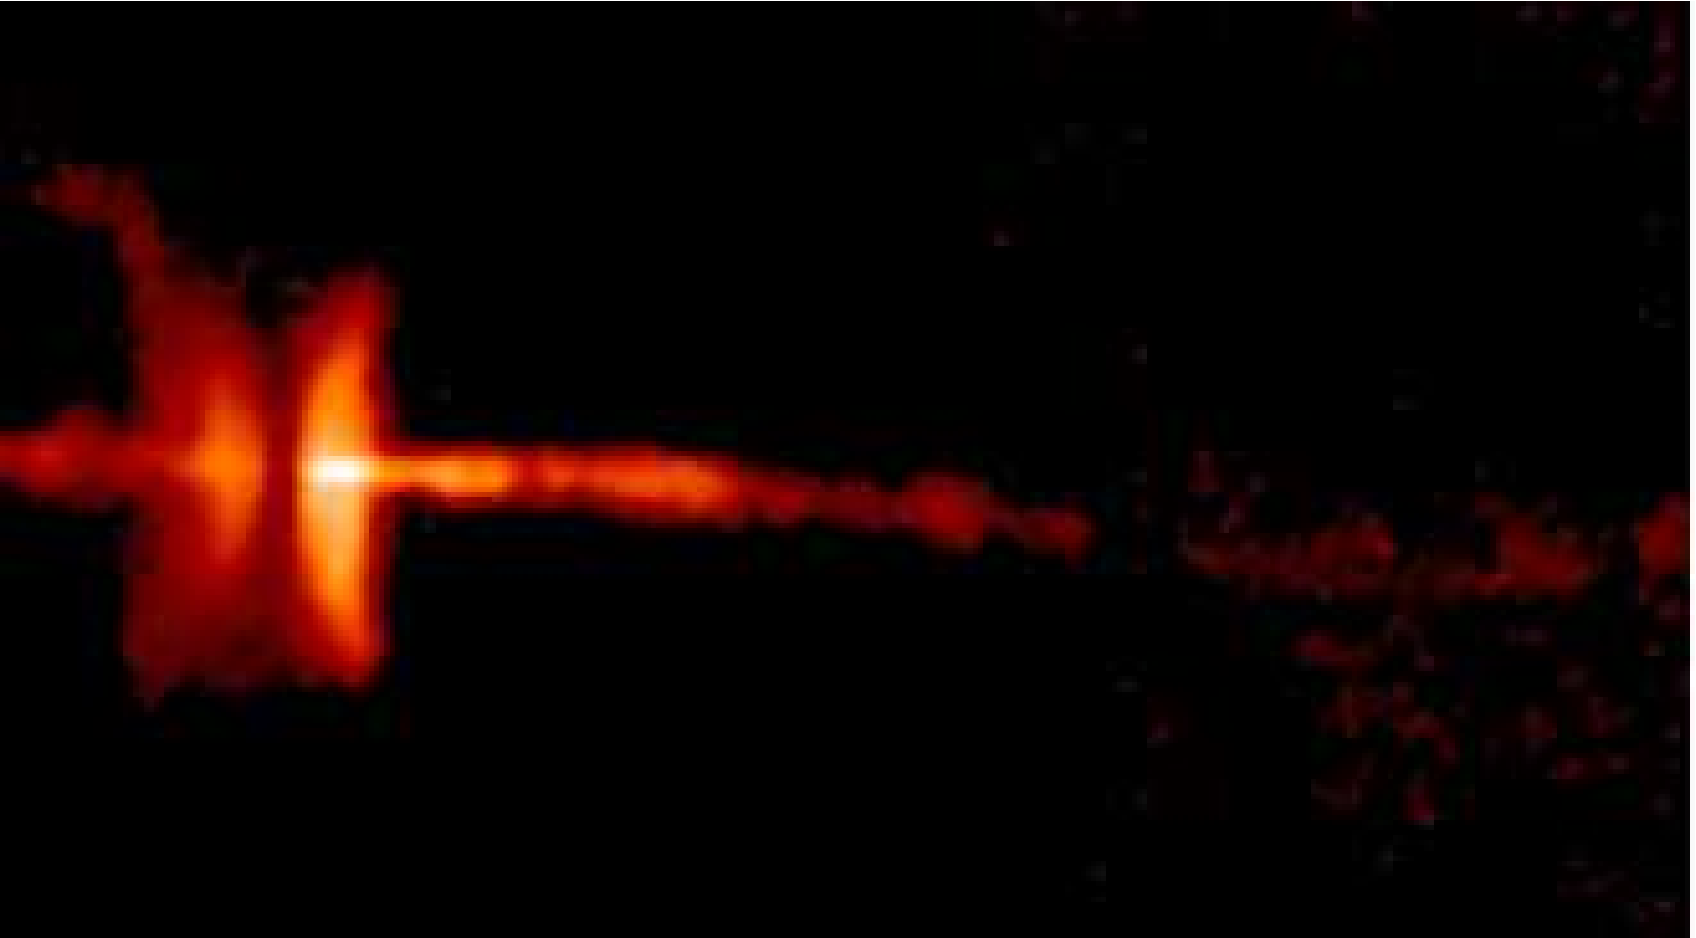
\includegraphics[width=8cm]{CollimatedJet}
\caption{
HH30, a high velocity (v$_{jet} \sim$ 200 km~s$^{-1}$), highly collimated (opening angle $\sim$ 2$^{\circ}$ degrees) jet from a young star.
Image from Alan Watson (UNAM, Mexico), Karl Stapelfeldt (JPL), John Krist (STSI) and Chris Burrows (ESA/STSI)
}
\label{fig:5-01}       % Give a unique label
\end{figure}


\subsection{Motivation: Circulation Model}
%\section{Motivation: Circulation Model}

\begin{figure}[t]
\centering
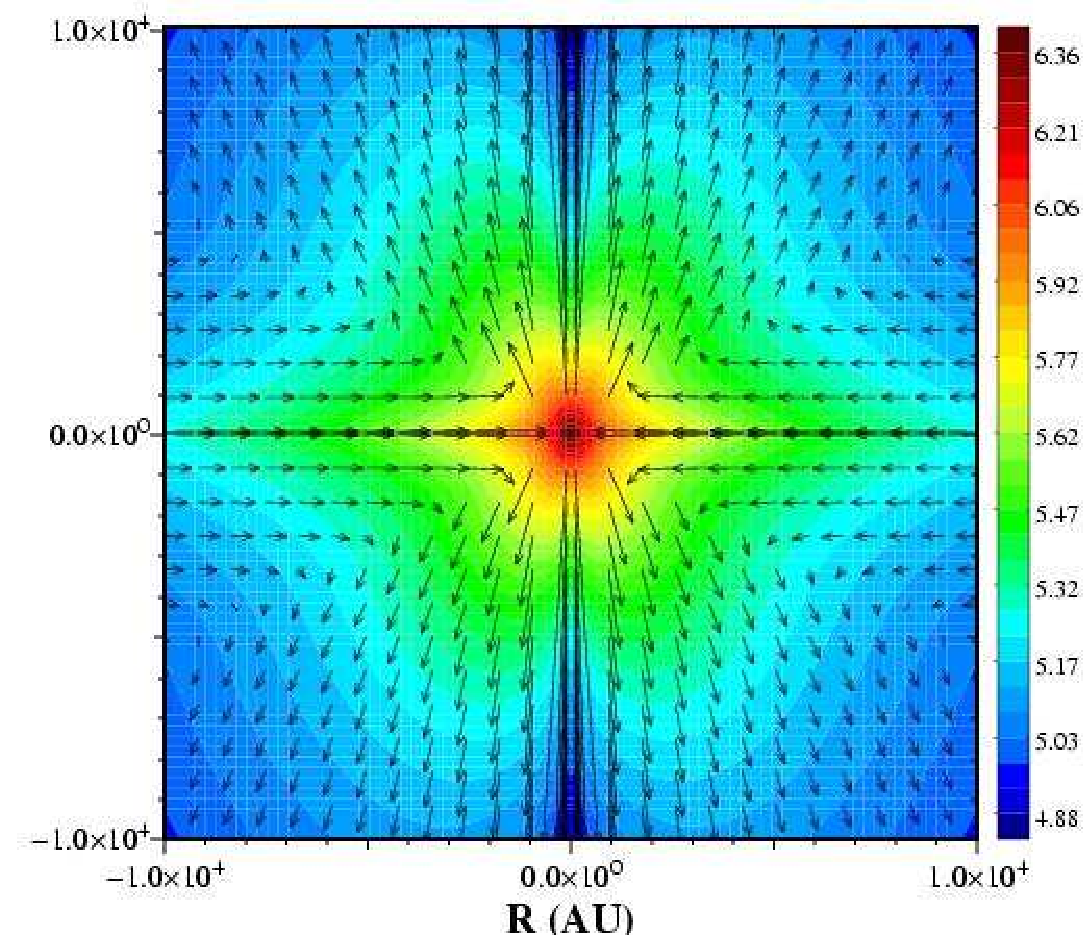
\includegraphics[width=8cm]{circulation}
\caption{
The circulation model: the densities are shown in log scale colour and the velocity field is shown by the arrows. From \citet{2006ApJ...637..798C}.
}
\label{fig:circulation}       % Give a unique label
\end{figure}

The circulation or transit flow model is an analytical self-similar solution to the steady-state MHD equations. 
\citet{1996MNRAS.281.1038F}, \citet{1999A&A...350..254L}, \citet{2002A&A...387..187L} and \citet{2006ApJ...637..798C} have solved the self similar equations.
They have shown a number of features including a strong density gradient towards the z-axis.
The density gradient is found for both weakly magnetised and strongly magnetised solutions.
The density gradient is naturally created by the infalling material encountering a higher thermal pressure near the central object causing the infall to deviate into an outflow.
%#causing gas to be pushed up along the axis.
The circulation model is one dimensional and collapses two spatial dimensions (r,$\theta$) onto one self-similar variable. 
%Hence it has a singularity at the axis and the solution may not be calculated on the axis. 
Hence the solution cannot strictly reach either the z-axis or the equator and can only be applied between $\theta_{max}$ and $\theta_{min}$, where ($\theta_{min} > 0$ and $\theta_{max} < \frac{\pi}{2}$).
Nevertheless the solutions indicate evidence for a density decrease towards the axis precisely where the jet will propagate.
%indicate there is a density gradient and it should be included in simulations.
The density gradient towards the z-axis as derived in the circulation model 
is shown in Figure \ref{fig:circulation} 
\citep{2006ApJ...637..798C}. 
The idea of the simulation is to launch a jet into the solution of the transit flow and see its effects on the jet morphology and dynamics.

\subsection{Motivation: Prehistory of Jets and Outflows from the Source}
%\section{Motivation: Prehistory of Jets}

The prehistory of outflows from the same source generates channels which affect the succeeding outflows from the same source.
%Quillen et al 
\citet{2005ApJ...632..941Q} show that such a channel will take $10^6$ years for the molecular cloud to diffuse back into the channel. Therefore the cavity will remain open long enough for successive outflows to propagate into and along it. 


%Close to sources, observations have shown strong energetic emission and strong ionisation, as measured by the ionisation fraction \citep{1999A&A...342..717B}. One potential source could be strong shocks due, for example, to recollimation.
\subsection{Recollimation}
Jets may be collimated by external hydrodynamic pressure or by the toroidal pressure of a wound-up magnetic field.
Far from the protostar the magnetic field diminishes by orders of magnitude and it is reasonable to assume that magnetic forces play a smaller role in recollimation at distances of $\sim 100$ AU. 
Some collimation of the jet may be caused by its environment; there are a
number of theories e.g. toroidal magnetic fields existing in the ambient medium, the pressure exerted by the molecular cloud collapsing
inwards, or just the presence of a cavity surrounded by dense walls
which force the jet to become collimated.  
As far back as \citet{1982ApJ...261..115K} and \citet{1989ApJ...344..404R} de Laval nozzles were thought to be responsible for the initial collimation of an
outflow.  
More recently \citet{1991A&A...252..718M,1992A&A...253..224I} and \citet{1992Natur.355..524I}
investigated ``shock-focused" inertial confinement, where oblique inward
facing shocks are produced by jet interaction with a toroidal density
distribution in the ambient medium \citep{1998ApJ...494L..79F} in the
context of planetary nebulae and \citet{1994A&A...290..643F} applied
this to jets in young stellar objects (YSOs).
\citet{1996ApJ...472..684F} (hereafter FM) modelled a central wind from
a YSO interacting with a toroidal density distribution.
\citet{1997MNRAS.292..795M} (hereafter MF) explored the same problem this time
including the effects of atomic radiative cooling.
\citet{2003ApJ...582..269G} (hereafter GFH) simulated wide-angle winds
interacting with a collapsing environment and a toroidal magnetic field.
\citet{2004ApJ...611..575O} (hereafter OLV) modelled the formation of a
jet by a de Laval nozzle effect, which includes lateral variations in
the magnetic field.  FM, MF and GFH all used 2D simulations, either
axisymmetric or spherically symmetric.  OLV performed a fully 3D
simulation however they used a magnetic field to perform the collimation
rather then a density gradient.  
%Rather than study the collimation of a spherical wind or bubble into a jet as has been studied in some of the previously cited work this chapter is concerned with recollimation of a jet by the ambient medium.  
In this chapter the possibility of additional collimation of a jet by a reduced density in the environment and the observational consequences to the underlying flow is investigated.


%\subsection{Parameter space study: axisymmetric models of evacuated cavities}


\section{Method}
\subsection{Numerical method}
In this study, we will primarily vary two parameters, the ratio of the jet density to ambient density 
$\eta$ and the reduction of density of the ambient medium in the centre of the cavity, the density decrement, $\delta$.
The parameter space is explored using the numerical code FLASH \citep{2002ApJS..143..201C}.
Using these results a larger simulation is carried out using the numerical code ATLAS described in Chapter 2.
%Two numerical codes are used, ATLAS (see Chapter 2) and FLASH \citep{2002ApJS..143..201C}.
The hydrodynamical equations are evolved in time, in 2.5D and 3D.
% want to model the collimation of jets, using a mechanism which is purely hydrodynamic and does not require the MHD approximations.
% want to see the full three-dimensional effect of the collimation therefore wish to use a numerical model which can efficiently model the large domain without unsustainable computational expense.



\subsection{System of equations}

The simulation code solves the ideal hydrodynamics (HD) equations.
The equations are expressed in terms of the 3 quantities (1 vector and two scalar) in addition to time t which are conserved in a volume:
density $\rho$, momentum, $\rho \mathbf u$, and energy density, $E$.


\begin{equation}
\frac{\partial \rho}{\partial t}+\nabla\cdot(\rho \mathbf u)=0
\end{equation}

\begin{equation}
\frac{\partial}{\partial t}\left(
\rho \mathbf u
\right)
+\nabla
\cdot
\left[
\rho \mathbf u \mathbf u
+\left(
p
\right)
\mathbf {{\overline {\overline I}}}
\right]
=0
\end{equation}



\begin{equation}
\frac{\partial E}{\partial t}
+\nabla
\cdot
\left[
\left( E + p\right) \mathbf{u}
\right] + L_{cooling} = 0
\end{equation}

\begin{equation}
E =
\frac{1}{2}\rho u^2 + 
\frac{p}{\gamma-1}
\end{equation}


$L_{cooling}$ represents the losses due to optically thin radiative cooling.
The units are chosen so that $\mathbf B$ absorbs a factor of $1/\sqrt {4 \pi}$.
The adiabatic index is $\gamma = 5/3$ for a monatomic gas throughout the simulations.
The equation of state is the ideal gas equation (p=nkT).
The same atomic radiative cooling function is used in both ATLAS and FLASH, and is described in Section \ref{ModellingtheMicrophysicsofAtomicRadiativeCooling}.

\subsection{Initial and boundary conditions} 
The values of the hydrodynamic
variables are set to those appropriate for Class I protostellar jets.  
The main parameters of these solutions are described in Table \ref{DensityGradientSims}.

\subsubsection{Initial conditions}
The
ambient medium is initialised with a uniform density ($1 \times
10^{-22}$~g~cm$^{-3}$) and temperature (10 K) and the jet is
initialised with the temperature of 1000K and density of $\eta\times10^{-22}~$g~cm$^{-3}$ and velocity of
300~km~s$^{-1}$, a typical YSO jet velocity
\citep{2000prpl.conf..815E}. 
For the 3D simulation only a velocity radial profile similar to the one used in Chapter \ref{BinaryJetsChap} is used.
The velocity radial profile is a positive cosine - with its maximum, v$_{jet}$ at r=0 in the jet centre, dropping to zero at r$_{jet}$. 

The evacuated cavity is parametrised using the sinusoidal function:

\begin{equation}
\rho\left( x \right) = {\rho}_0 \left( \frac{\delta+1}{2 \delta} \right) \left(1 + \cos \left( \frac{\pi}{2} \frac{ x}{r_{jet}}
\right)
 \right)
\end{equation}


where the density decrement, $\delta$ is the parameter chosen to represent the size of the cavity, $\delta=$1, or 10.
%Hydrodynamic equilibrium is preserved by varying the pressure in a similar fashion.
% can calculate the speed of sound in the medium $c=\sqrt {\gamma p /\rho} = 5.25$~km~s$^{-1}$. 
%JThe Mach number of the jet is $M_{jet} = M_{ambient} = 57.1$ with respect to the both jet and the ambient medium, since they have a common density and pressure.



\begin{table}
\begin{center}
\begin{tabular}{l r}
%Domain & $-0.166 $pc$<x<0.166$ pc \\
% &  $0<y<0.332 $pc$, -0.166 $pc$<z<0.166$ pc \\
% Coarsest grid    & $\Delta x=\Delta y=\Delta z=0.166$ pc \
Domain &  $8\times10^{16}$cm $\times $ $ 3.2\times10^{17}$cm \\
 Jet velocity   & $v_{jet}=300~$km~s$^{-1}$ \\
 Jet density      & $\rho_{jet}=1\eta\times10^{-22}~$g~cm$^{-3}$ \\
 Ambient density  & $\rho_a=1\times10^{-22}~$g~cm$^{-3}$ \\
 Jet Temperature     &$T_{jet}= 10^3 K$ \\
 Jet Radius     &$r_{jet}= 1\times10^{16}$cm \\
 Ambient Temperature &$T_a= 10 K$ \\
 %Finest grid &   $\Delta x=\Delta y=\Delta z=0.0026$ pc(5 levels) \\
 \end{tabular}
 \caption{Parameters used in the numerical calculations}
 \label{DensityGradientSims}
 \end{center}
 \end{table}


\subsubsection{Boundary conditions}

For the 3D simulation, the boundary conditions are inflow for $r<r_{jet}$, reflecting for $r>r_{jet}$ along the inner $r$-boundary ($z$=0) and outflow along all other boundaries.

For the axisymmetric simulations, the boundary conditions are identical, except for an extra reflecting boundary condition on the $z$-axis.


\section{Results}

\subsection{Parameter space exploration}

A jet entering an evacuated cavity is modelled.
The jet is forced inwards by the steep
density gradient of its environment.  
%Three different types of ambient
%background were used - the standard case of a constant density ambient
%medium (hereafter CDAM) a shallow and a steep gradient.
The parameters varied are, the density ratio, $\eta$ and the density decrement, $\delta$, which is defined above.
The effects of rapid velocity variation (pulsing) and radiative cooling are examined.

\begin{table}
\begin{center}
\begin{tabular}{l c c c}
\hline
       & $\eta$ & Cooling & Pulsed\\
\hline
 Case I &   10    &  N & Y\\
\hline
 Case II &   0.1  & N & Y \\ 
\hline
 Case III &   1   &  Y & N\\
\hline
 Case IV &   1   & Y & Y\\
\hline
 \end{tabular}
 \caption{Parameter Space}
\label{Parameter Space}
 \end{center}
 \end{table}


\subsection{Case I: Pulsed, overdense adiabatic jets in cavities}

\begin{figure}[t]
\begin{center}
   \begin{minipage}[t]{.48\linewidth}
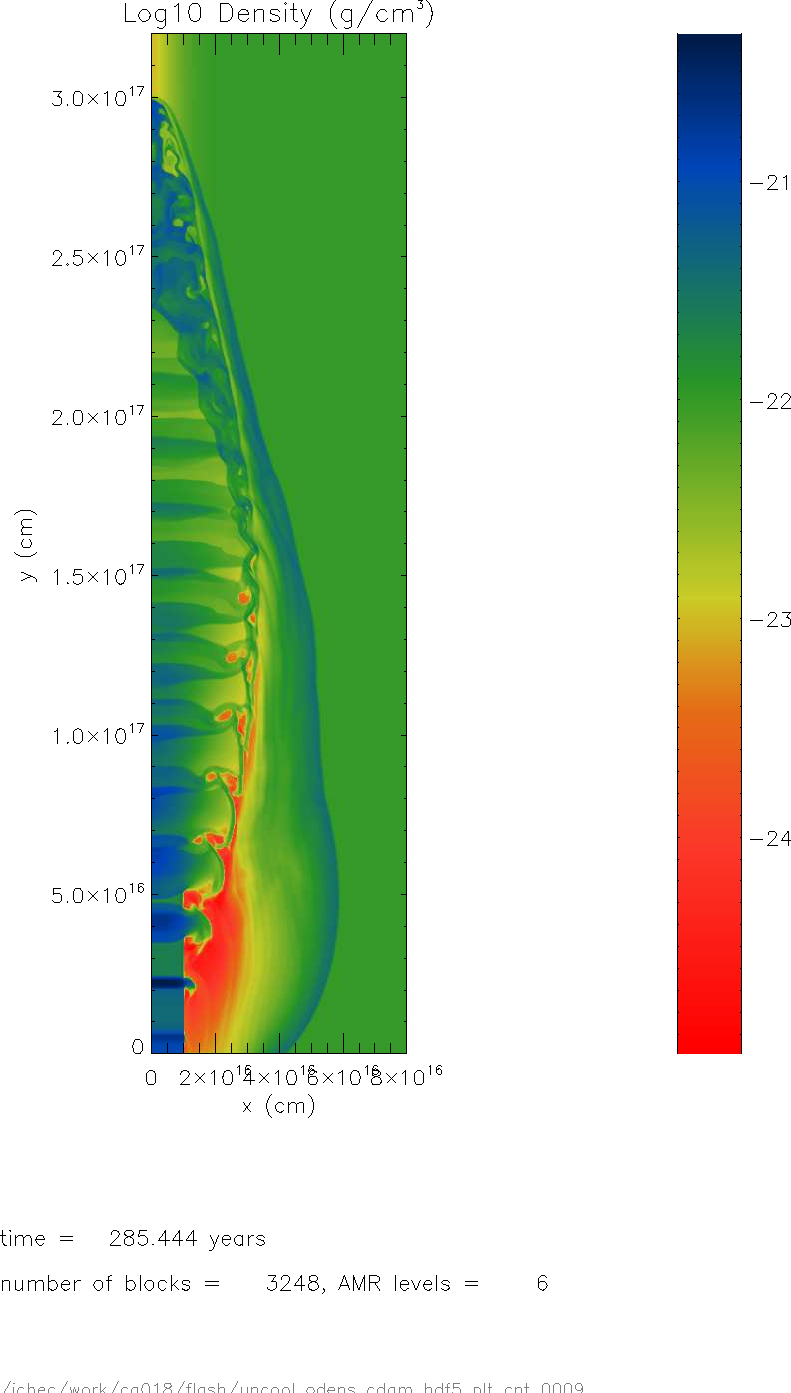
\includegraphics[width=8cm]{flash_evac_cav1}
   \end{minipage} 
   \begin{minipage}[t]{.48\linewidth}
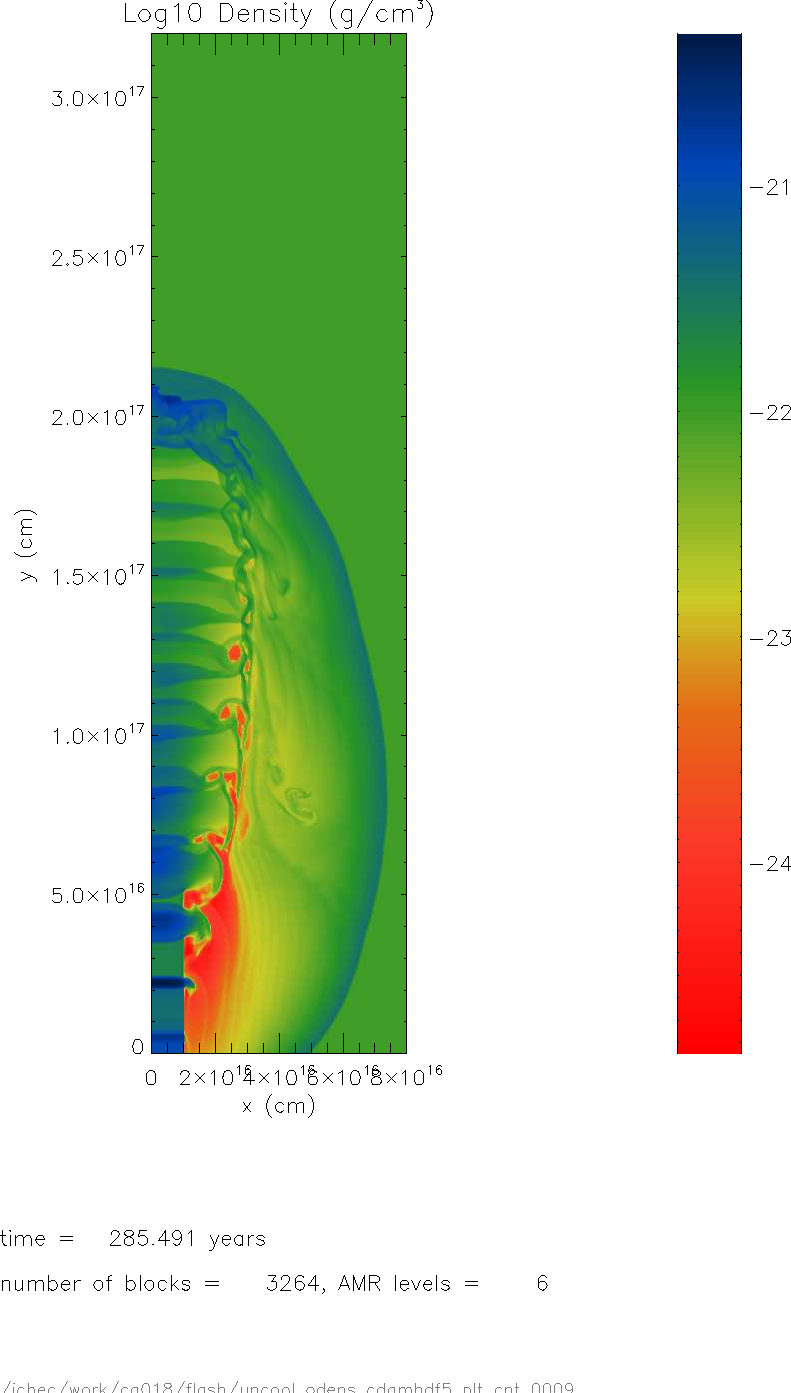
\includegraphics[width=8cm]{flash_evac_cav2}
   \end{minipage} 
\caption{
Overdense ($\eta$=10), 300 km~s$^{-1}$, Mach 800 adiabatic jet, velocity-pulsed with an amplitude of 30\% and a period of 9.6 years ($3\times10^8$ s) injected into 
(left panel)
an evacuated cavity, with density decrement, $\delta$=10.
Strong recollimation and rapid acceleration are evident, compared with the 
right panel, which shows an identical jet in constant density ambient medium (CDAM).
The box is an axisymmetric rectangle 
3$\times$10$^{17}$ cm by
8$\times$10$^{16}$ cm.
An adaptive grid is used with 6 levels of refinement, and a resolution equivalent to 256x1024-sized uniform mesh.
%The finest resolution is then 3.125$\times$10$^{14}$ cm.
}
\label{fig:flash:eta:10}       % Give a unique label
\end{center}
\end{figure}


The first case is an overdense jet propagating into an evacuated environment. 
(see Figure \ref{fig:flash:eta:10}).
%The jet has a jet-to-ambient Mach number of 800 and is injected already collimated into a constant density ambient medium.
This case includes two simulations with a constant density ambient medium and a density decrement of 10.
In both simulations the jet was initialised as cylindrical, with a nominal Mach number with respect to the ambient sound speed of 800.
The inlet velocity is pulsed with an amplitude of 30\% in order to reproduce the knots visible in observations.
It expands in typical adiabatic fashion and has a low length-to-width ratio $\sim$2.5.
The effect of adding an evacuated cavity, with a density decrement, $\delta$ = 10 is to produce increased collimation well behind the bow shock.
The length-to-width ratio is $\sim$5.
The jet is compressed toward the axis and small structures are visible.
However behind the head of the jet the jet evolves similarly to the CDAM jet, so the effect is only a transient one, and only the first few ``knots'' see the cavity.
The dense ``interstellar bullets'' at the head of the jet effectively plough the cavity structure out of the way.


\subsection{Case II: Pulsed, underdense adiabatic jets in cavities}

\begin{figure}[t]
\begin{center}
   \begin{minipage}[t]{.48\linewidth}
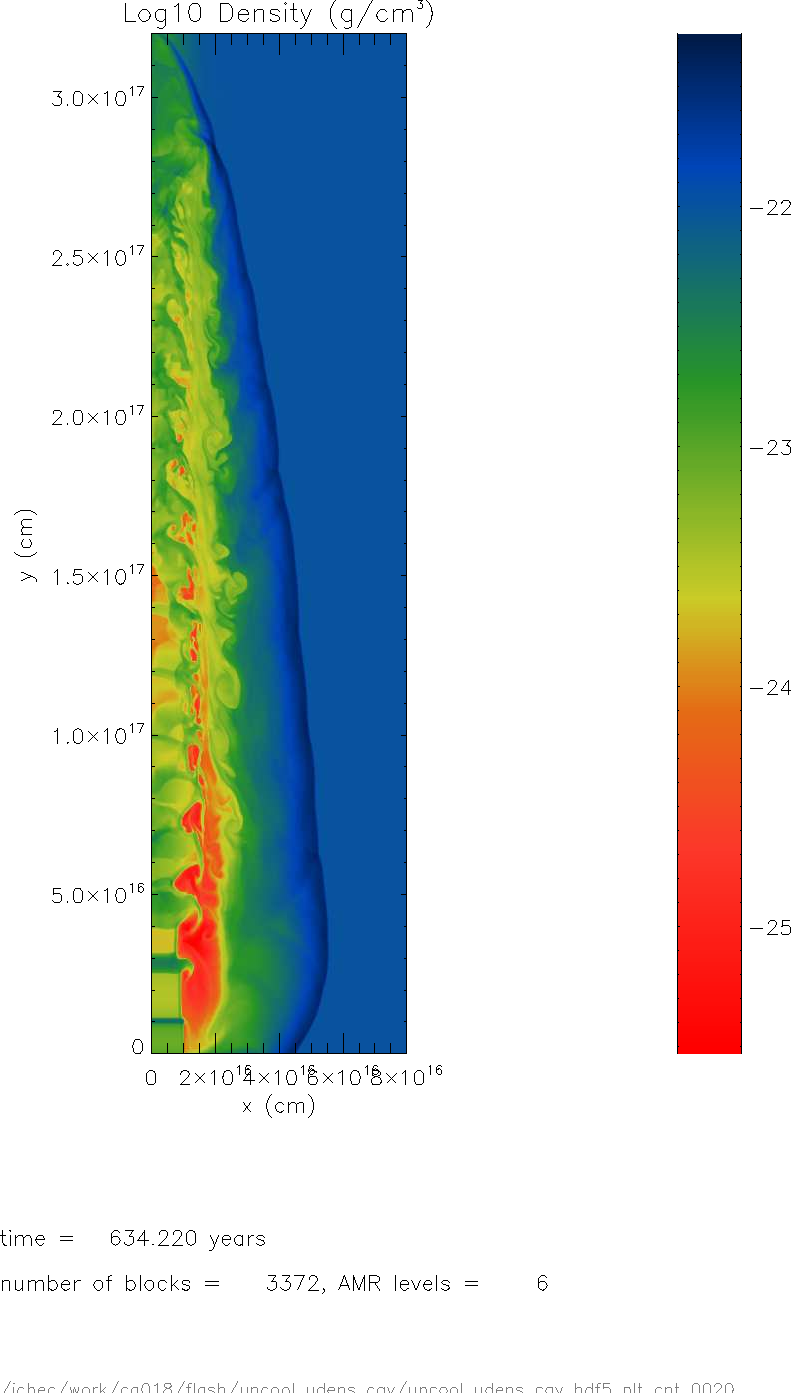
\includegraphics[width=8cm]{flash_ud10_cav}
   \end{minipage} \hfill
   \begin{minipage}[t]{.48\linewidth}
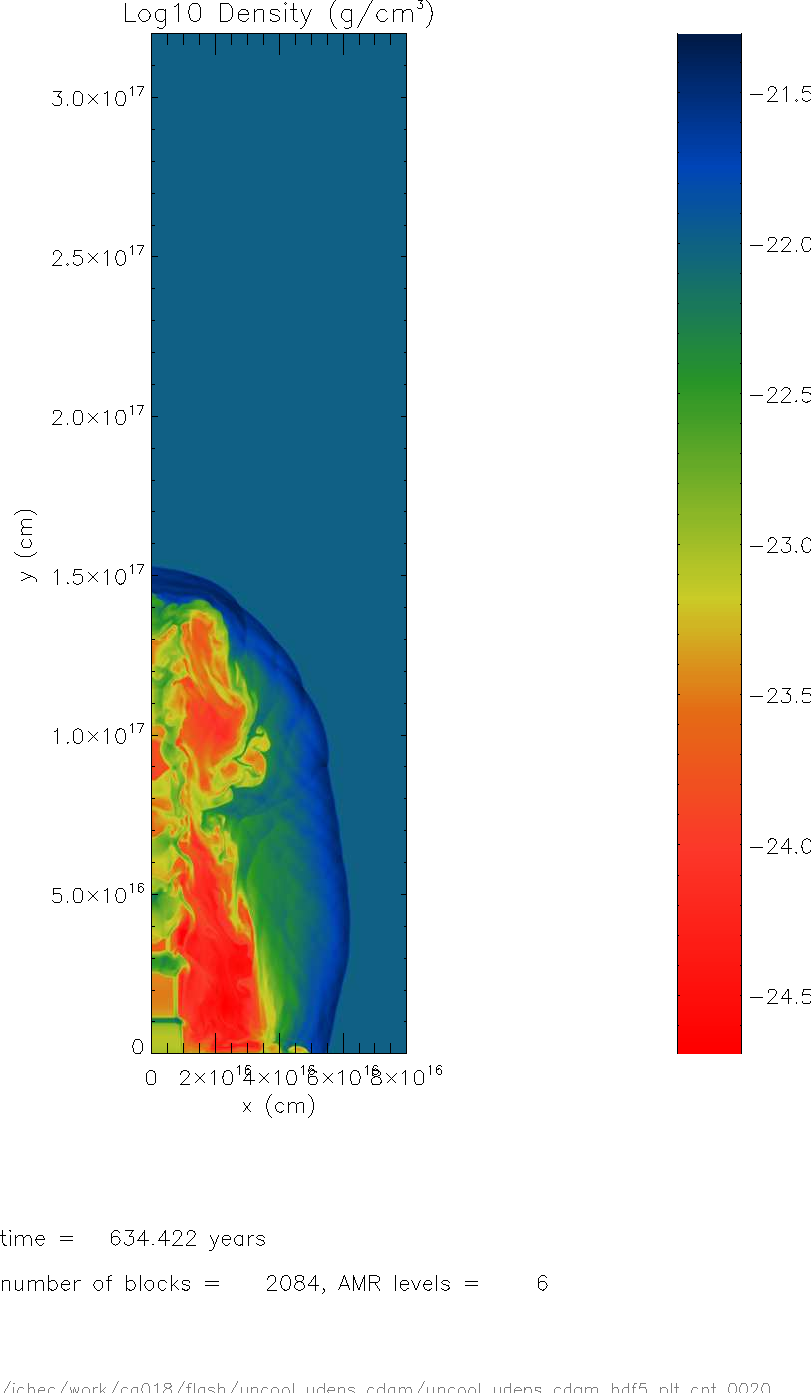
\includegraphics[width=8cm]{flash_ud_cav}
   \end{minipage} \hfill
\hfill
\caption{
Underdense ($\eta$=0.1), 300 km~s$^{-1}$, Mach 800  adiabatic jet, velocity-pulsed with an amplitude of 30\% injected into
(left panel)
an evacuated cavity with density decrement, $\delta$=10, 
(right panel)
a constant density ambient medium (CDAM).
The acceleration is most pronounced in this case.
}
\label{fig:flash:eta:0.1}       % Give a unique label
\end{center}
\end{figure}

%Recollimation - in Figure \ref{fig:2} a jet is shown travelling through an evacuated cavity at different stages of evolution. The jet clearly narrows towards the end point.  For comparison an identical jet is shown without the gradient in ambient density - and note the much less pronounced recollimation.


The second case was an underdense jet propagating into an evacuated environment. 
(see Figure \ref{fig:flash:eta:10}).
%The jet has a jet-to-ambient Mach number of 30 and is injected already collimated into a constant density ambient medium.
%The inlet velocity is pulsed with an amplitude of 30\% in order to reproduce the knots visible in observations.
%It expands in typical adiabatic fashion and has a low length-to-width ratio.
%The effect of adding an evacuated cavity, with a $\delta$ of 10 is to produce increased collimation \emph{in the head} of the jet. The jet is compressed toward the axis and small structures are visible.
%However behind the head of the jet the jet evolves similarly to the CDAM jet, so the effect is only a transient one, and only the first few ``knots'' see the cavity.
This simulation has much in common with the first case. However for the underdense jet case, the jet behaves more like an expanding bubble and is more strongly and dramatically affected by the cavity, the aspect ratio increases from 2.5 in the CDAM to 6.4 in the evacuated case.
The jet in the cavity has a bow shock advance speed of 0.5$v_{jet}$, and
at t=634 years, the cavity jet has already crossed the grid, whereas the CDAM jet has an advance speed of only 0.25 $v_{jet}$.
Characteristics associated with Kelvin-Helmholtz instabilities are highly visible in the cocoon.
The initially flat, top-hat profile pulses become distorted as the jet propagates further into the cavity.


\subsection{Case III: Steady, radiatively cooling jet in cavity}

\begin{figure}[t]
\begin{center}
   \begin{minipage}[t]{.48\linewidth}
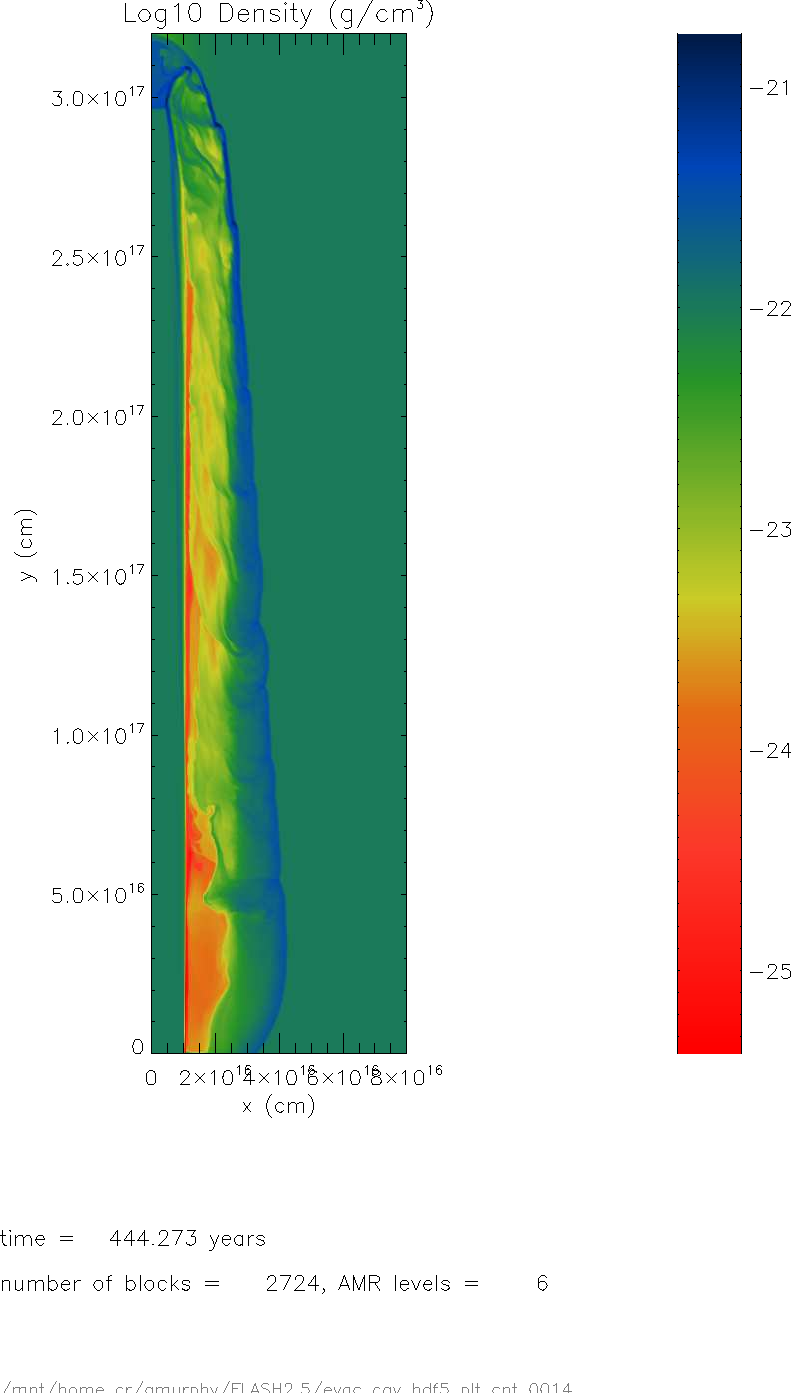
\includegraphics[width=8cm]{cool_cav}
   \end{minipage} \hfill
   \begin{minipage}[t]{.48\linewidth}
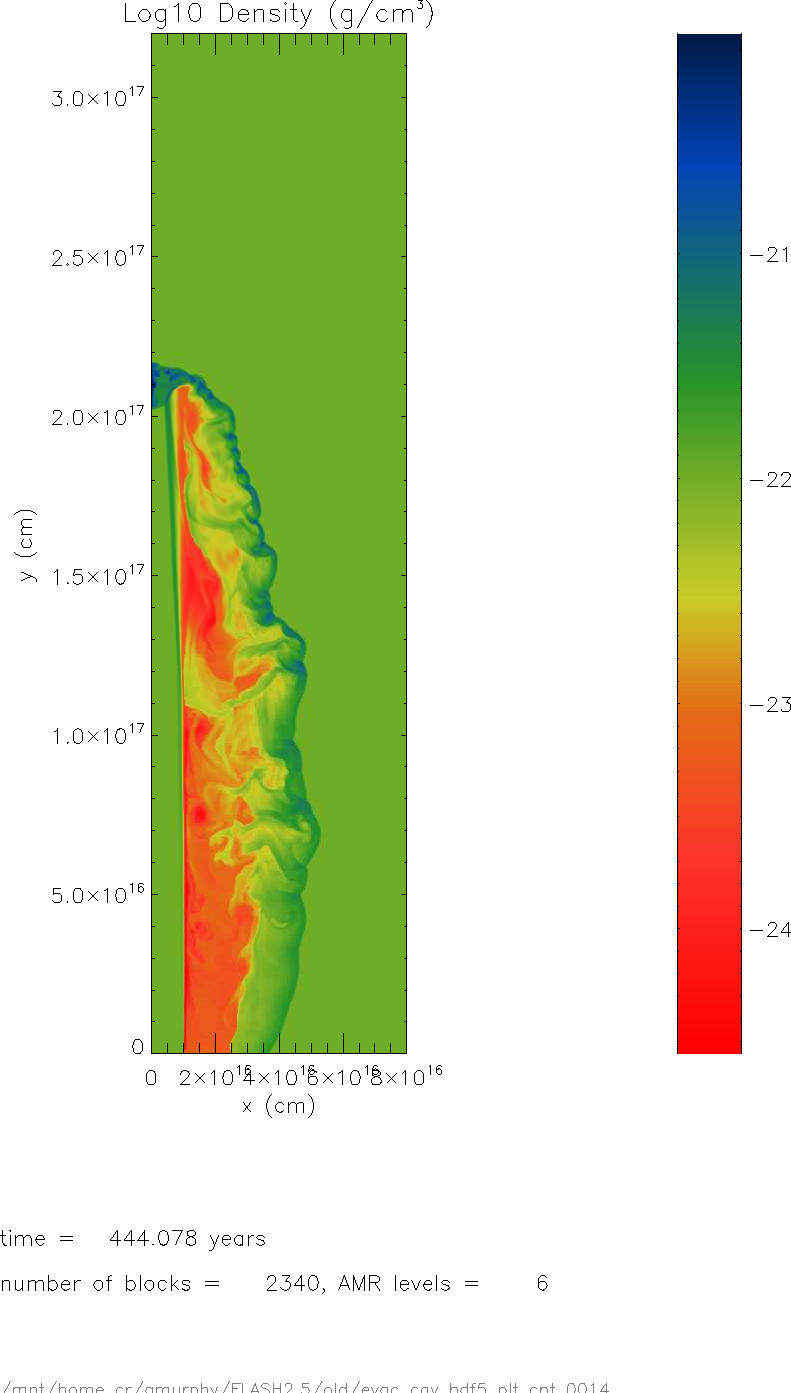
\includegraphics[width=8cm]{cool_cdam}
   \end{minipage} \hfill
\hfill
\caption{
Left panel:
Steady, radiatively-cooled jet in evacuated cavity, with density decrement, $\delta$=10 and $\eta$=1
Right panel: 
Identical jet in constant density ambient medium, with $\eta$=1
With strong radiative cooling typical of protostellar jets, recollimation is less apparent.
The cooling instabilities are much less evident.
}
\label{fig:flash:cool}       % Give a unique label
\end{center}
\end{figure}


In the third case strong radiative cooling has been enabled in the simulation.
For clarity, the 30\% variation in the inlet velocity has been removed.
The effect of the evacuated cavity on cooling instabilities inside the cocoon and on the bow shock surface is shown in Figure \ref{fig:flash:cool}.
The pressure gradient compresses the cocoon and narrows the cavity swept out by the fast jet.
The distinctive tendril features evident in right panel of Figure \ref{fig:flash:cool} (between $5\times10^{16}$~cm and $1\times10^{17}$~cm ) are absent in the cavity case.
The strong acceleration of the bow shock is still present.
The effect of the radiative cooling is to drain thermal pressure from the cocoon and collapse the bow shock.
The radiative jets are thus more narrow, the aspect ratios increase to 8 for the cavity case and 4.4 for the CDAM case.
There is a relative decrease in the amount of collimation from the adiabatic to the non-adiabatic case, which could possibly be attributed to the formation of a dense plug of material at the head of the jet, which cannot be much further compressed by the ambient medium 
(visible on the y-axis at $3\times10^{17}$~cm).


%\begin{figure}[t]
%\centering
%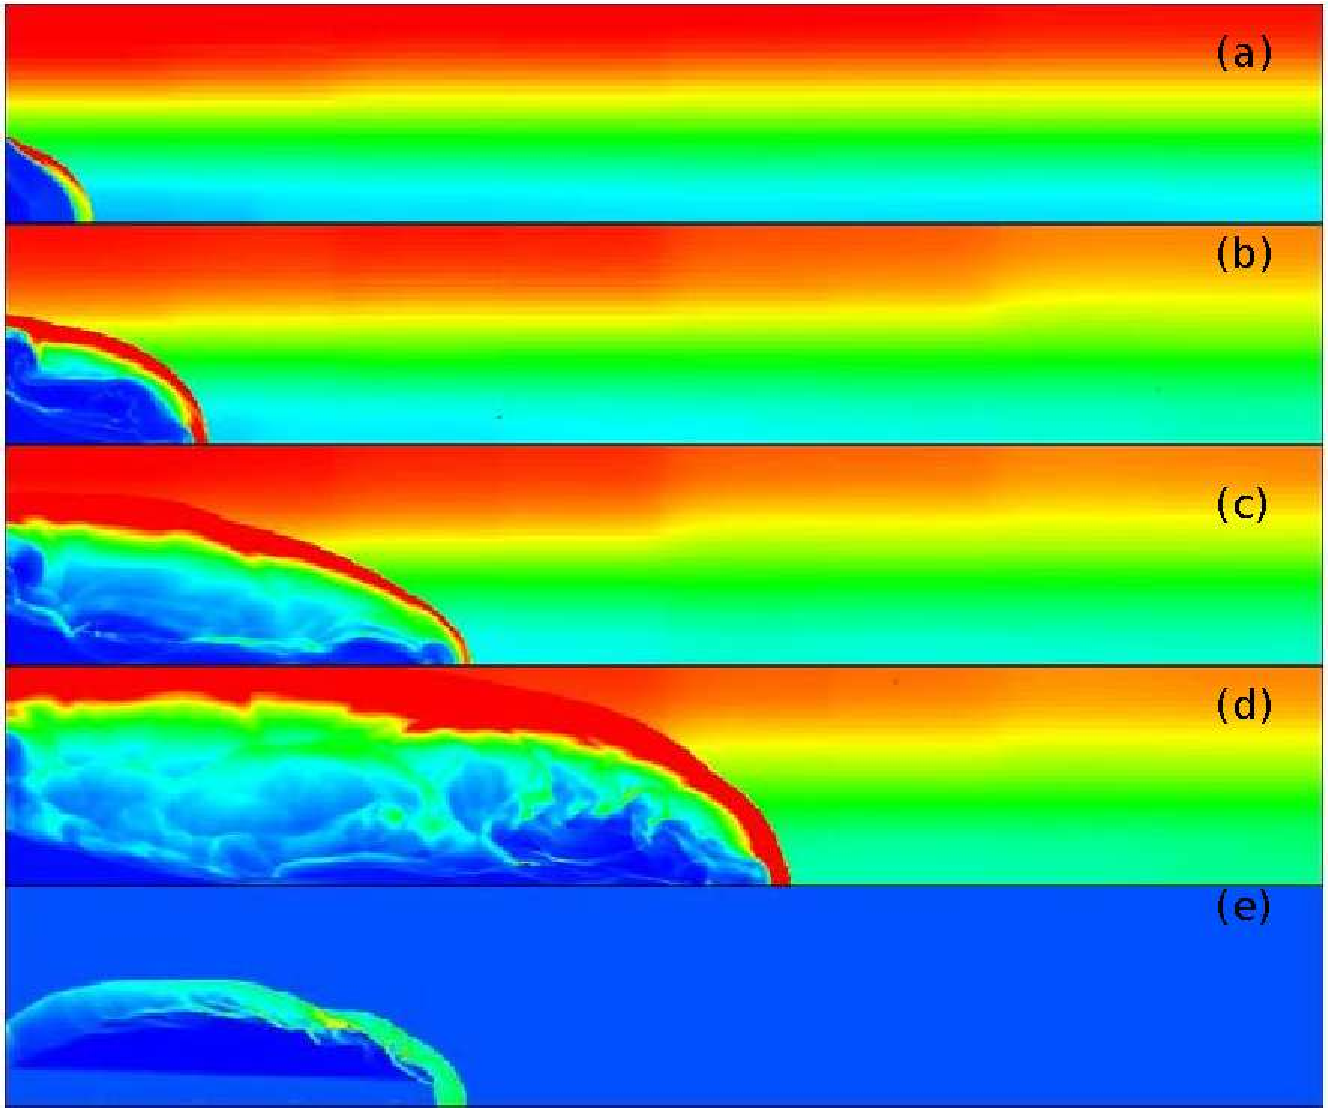
\includegraphics[width=8cm]{major_evac}
%\caption{
%Simulation results for jet in evacuated cavity: Density profile of 300 km s$^{-1}$ jet at $t$=126.8 (a), 317 (b), 634 (c), 1268 (d) $\mathrm{years}$. The model is slab-symmetric.
%For comparison (e) the density profile of 300 km s$^{-1}$ jet at $t=723\mathrm{~years}$ without evacuated cavity is shown.
%}
%\label{fig:2}       % Give a unique label
%\end{figure}


\subsection{Case IV: Pulsed, non-adiabatic jet in cavity}


\begin{figure}[t]
\begin{center}
   \begin{minipage}[t]{.48\linewidth}
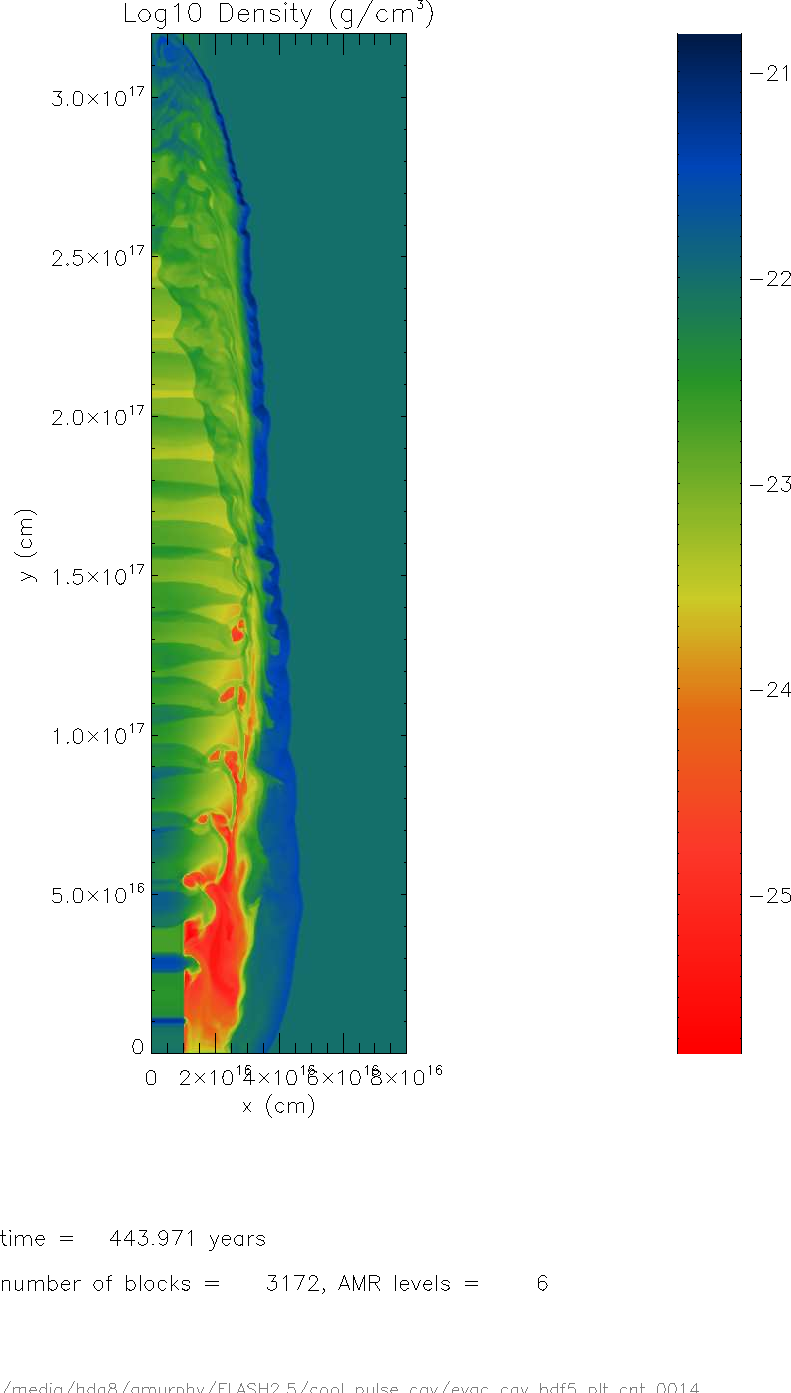
\includegraphics[width=8cm]{cool_pulse_cav}
   \end{minipage} \hfill
   \begin{minipage}[t]{.48\linewidth}
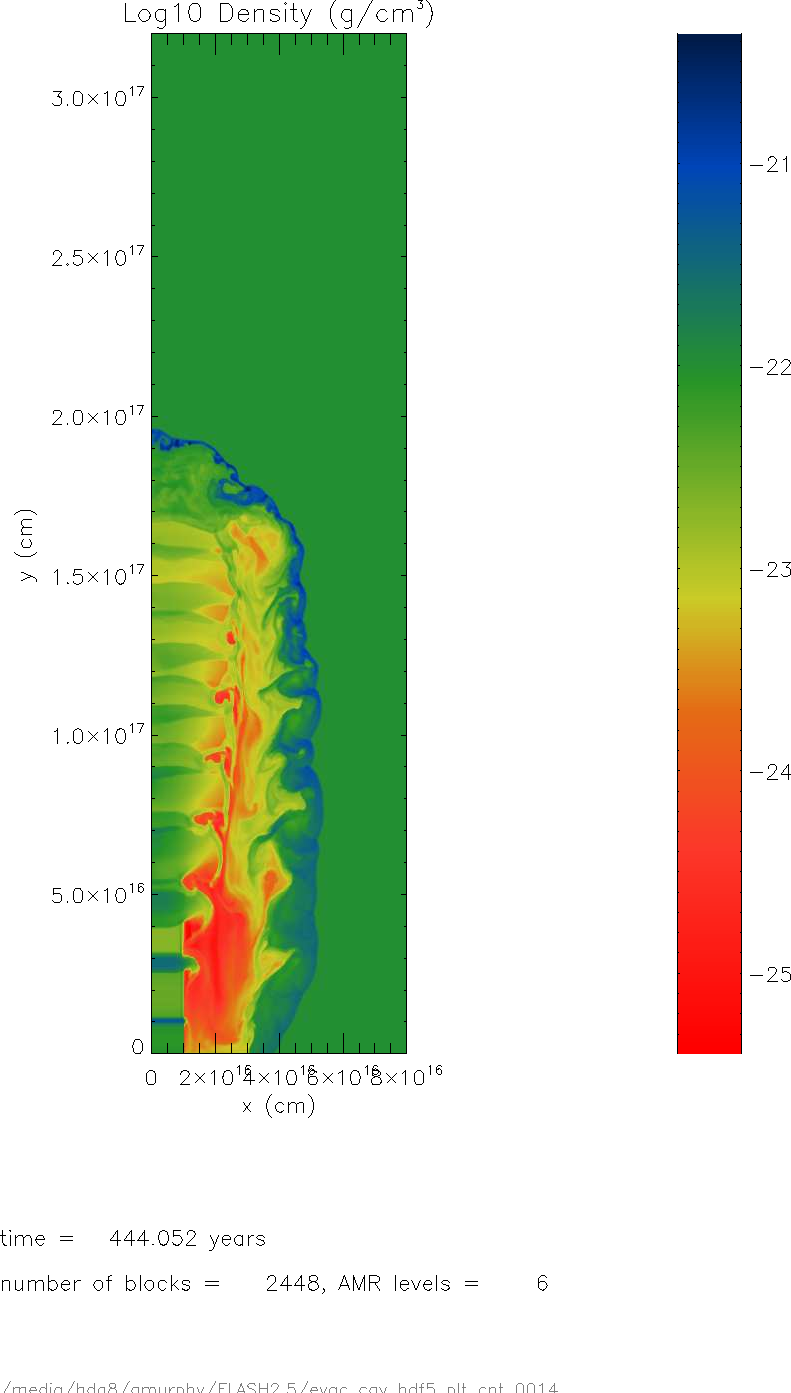
\includegraphics[width=8cm]{cool_pulse_cdam}
   \end{minipage} \hfill
\hfill
\caption{
Left panel:
Jet in evacuated cavity, with density decrement, $\delta$=10 and $\eta$=1
Right panel: 
Jet in constant density ambient medium, with $\eta$=1
With strong radiative cooling typical of protostellar jets, recollimation is less apparent.
The cooling instabilities are much less evident.
}
\label{fig:flash:cool_pulse}       % Give a unique label
\end{center}
\end{figure}



In the fourth case strong radiative cooling has been enabled in the simulation.
The 30\% variation in the inlet velocity has been restored.
A much more varied morphology is present in both the CDAM and the cavity case.
The aspect ratio increases from 4 to 6.1 in the evacuated case.


\subsection{Pulsed, non-adiabatic, three-dimensional jet in cavity}

Using the code ATLAS (see Chapter \ref{NumericalMethod}) a full three-dimensional simulation is performed.
In the 3D case the resolution is lower than can be achieved in 2.5D.
As a result the jet appears smoother and less instabilities.
The comparison between the cavity and CDAM jets again shows the basic differences of acceleration, cooling and recollimation (see Figure \ref{fig:3DDensity}).
By calculating the emissivity in each cell and integrating through the 3D domain, emission maps of the H$\alpha$ line are produced.
%The low resolution introduces some false structures into the emission map images.
In the 3D simulation with the density decrement of $\delta$=10 shown in Figure \ref{fig:3DDensity} the jet narrows sufficiently so that it is only spanned by 20 or so cells. This results in some false structures which are visible in the lower part of the emission map (Figure \ref{fig:3DEmission}).
%As a control for comparison a jet propagating into an unevacuated medium is used.  The standard case of a jet propagating in a CDAM is shown in Figure \ref{fig:11}. The jet has a velocity of 





%\begin{figure}[t]
%\centering
%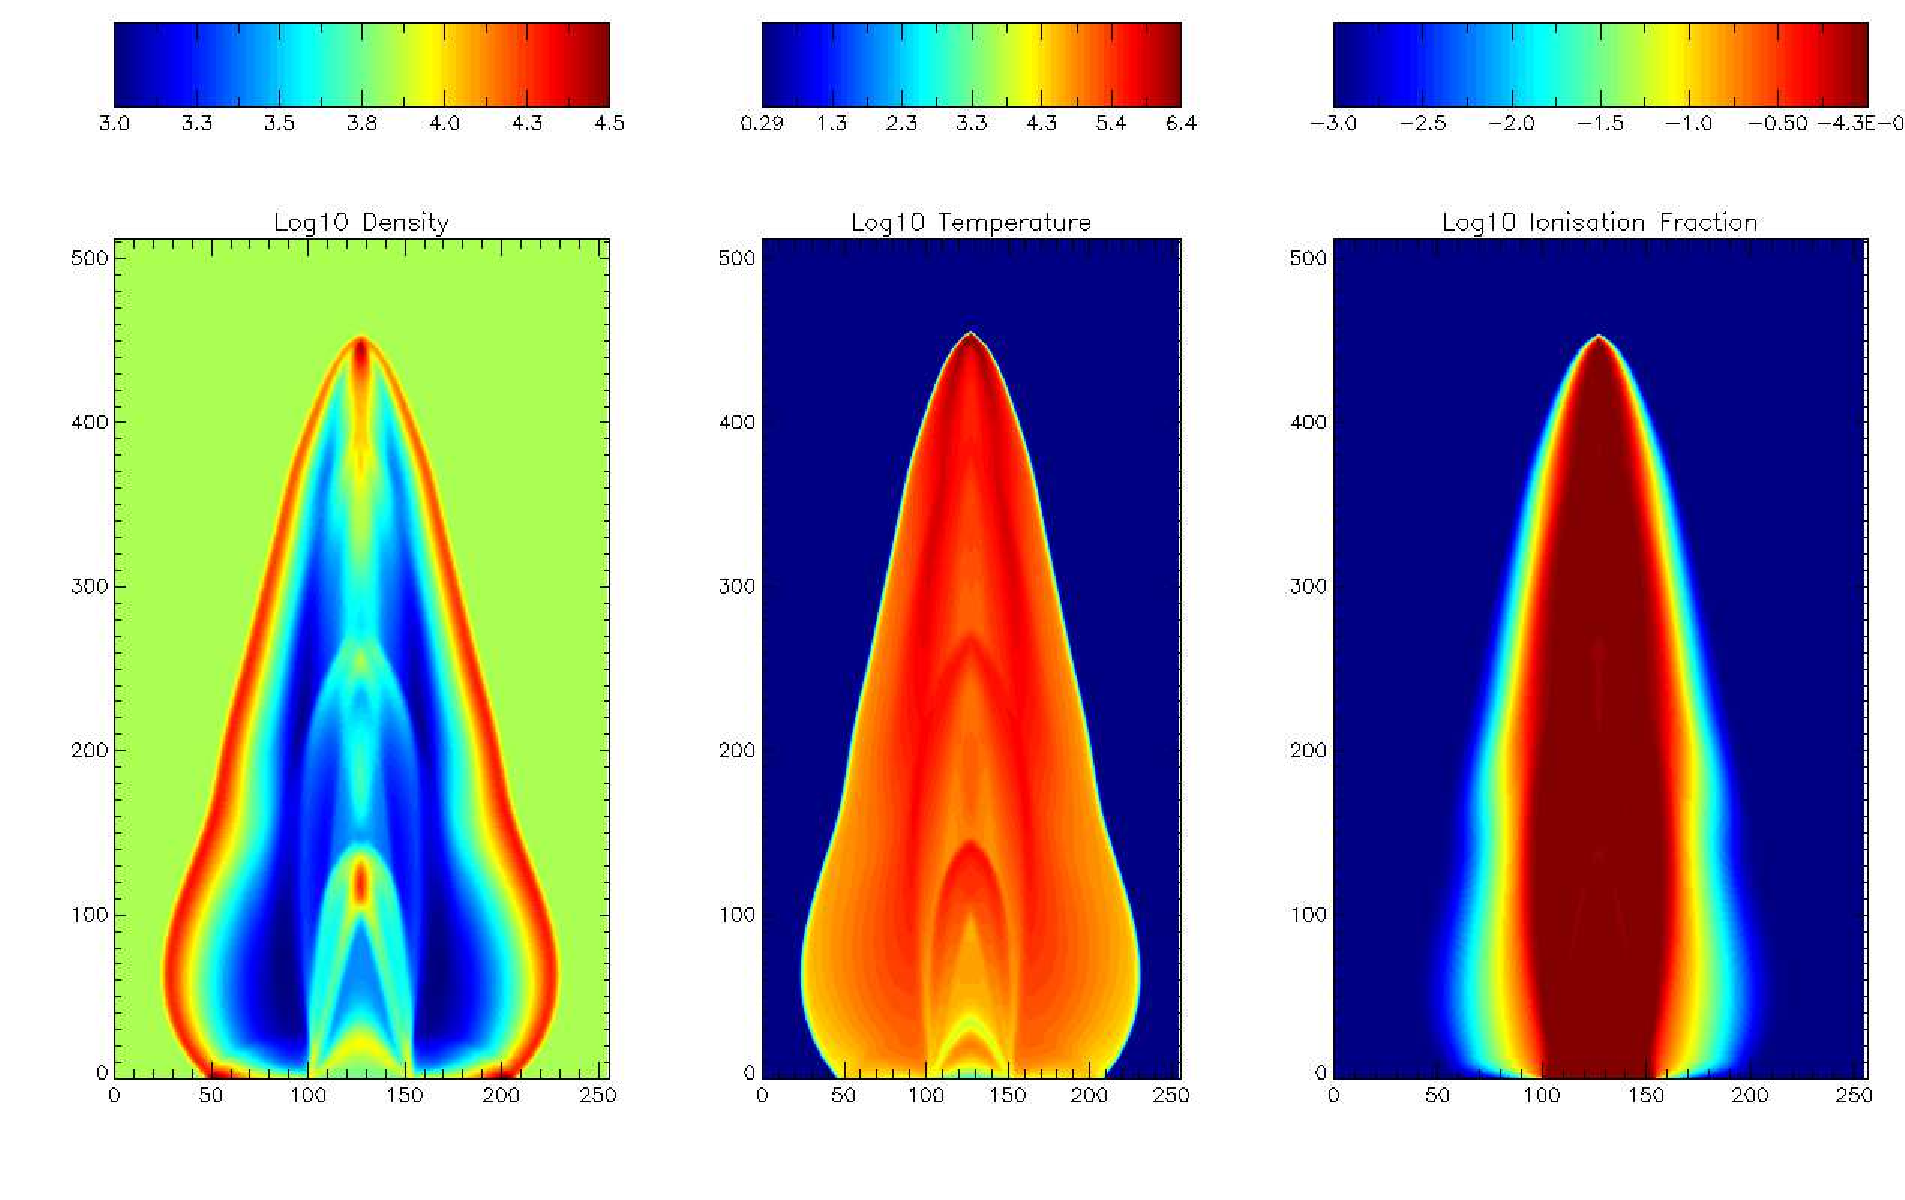
\includegraphics[width=9cm]{3d_cut_no_grad}
%\caption{
%Slice across 3d logarithmic density contours for 300~km~s$^{-1}$ purely hydrodynamical jet with atomic radiative cooling at $t=1065.12$ years.
%The source is pulsed with a 30\% variation in velocity every 100 years.
%The jet is overpressured with respect to the ambient medium.
%}
%\label{fig:11}       % Give a unique label
%\end{figure}


%\subsection{Case II}

%In Figure \ref{fig:13} the two major changes brought about by the ambient medium are shown, the acceleration of the jet and the collimation.

%\begin{figure}[t]
%\centering
%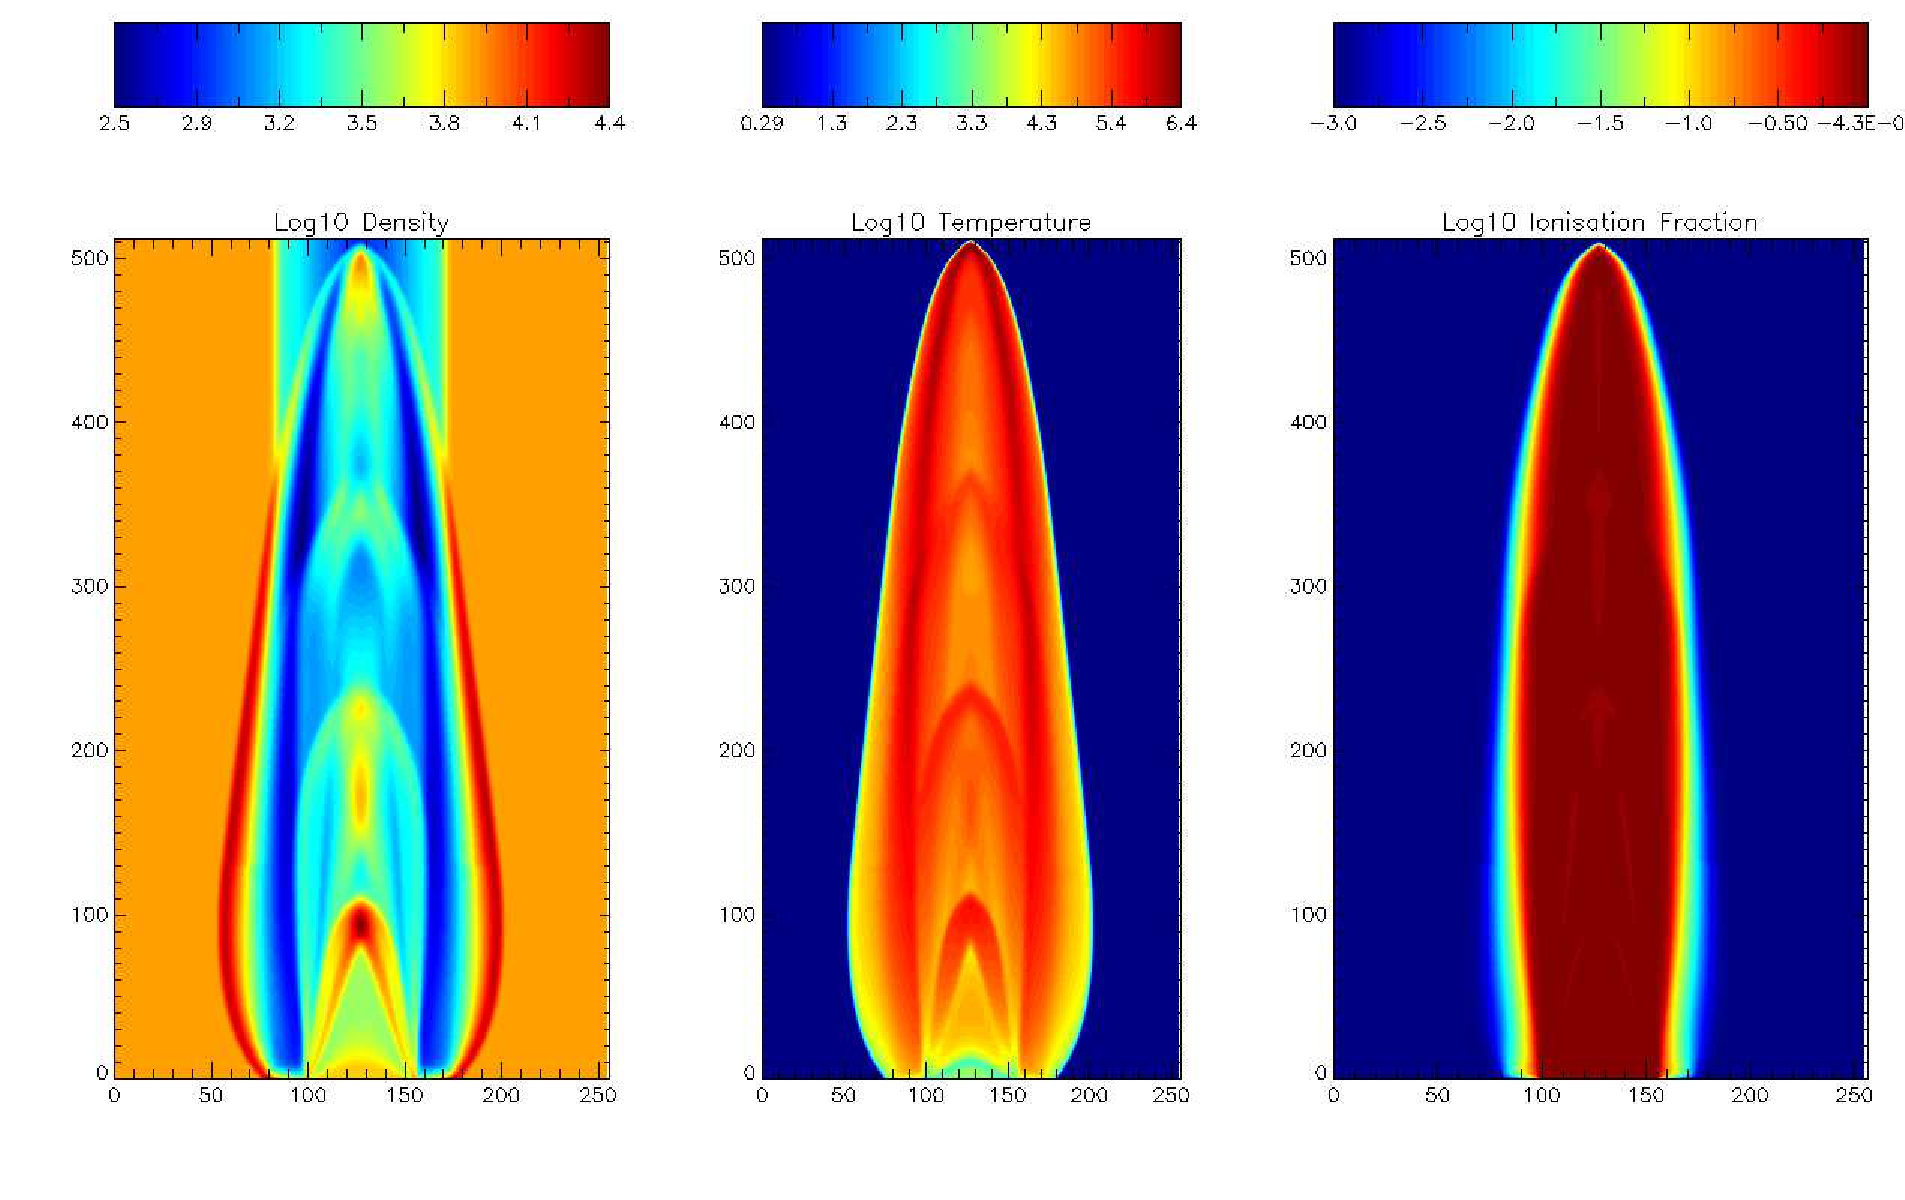
\includegraphics[width=9cm]{3d_cut_grad}
%\caption{
%Slice across 3d logarithmic density contours for 300~km~s$^{-1}$ purely hydrodynamical jet with atomic radiative cooling at $t=1065.12$ years.
%Further details are the same as in Figure \ref{fig:11}
%}
%\label{fig:13}       % Give a unique label
%\end{figure}




%\begin{figure}[t]
%\centering
%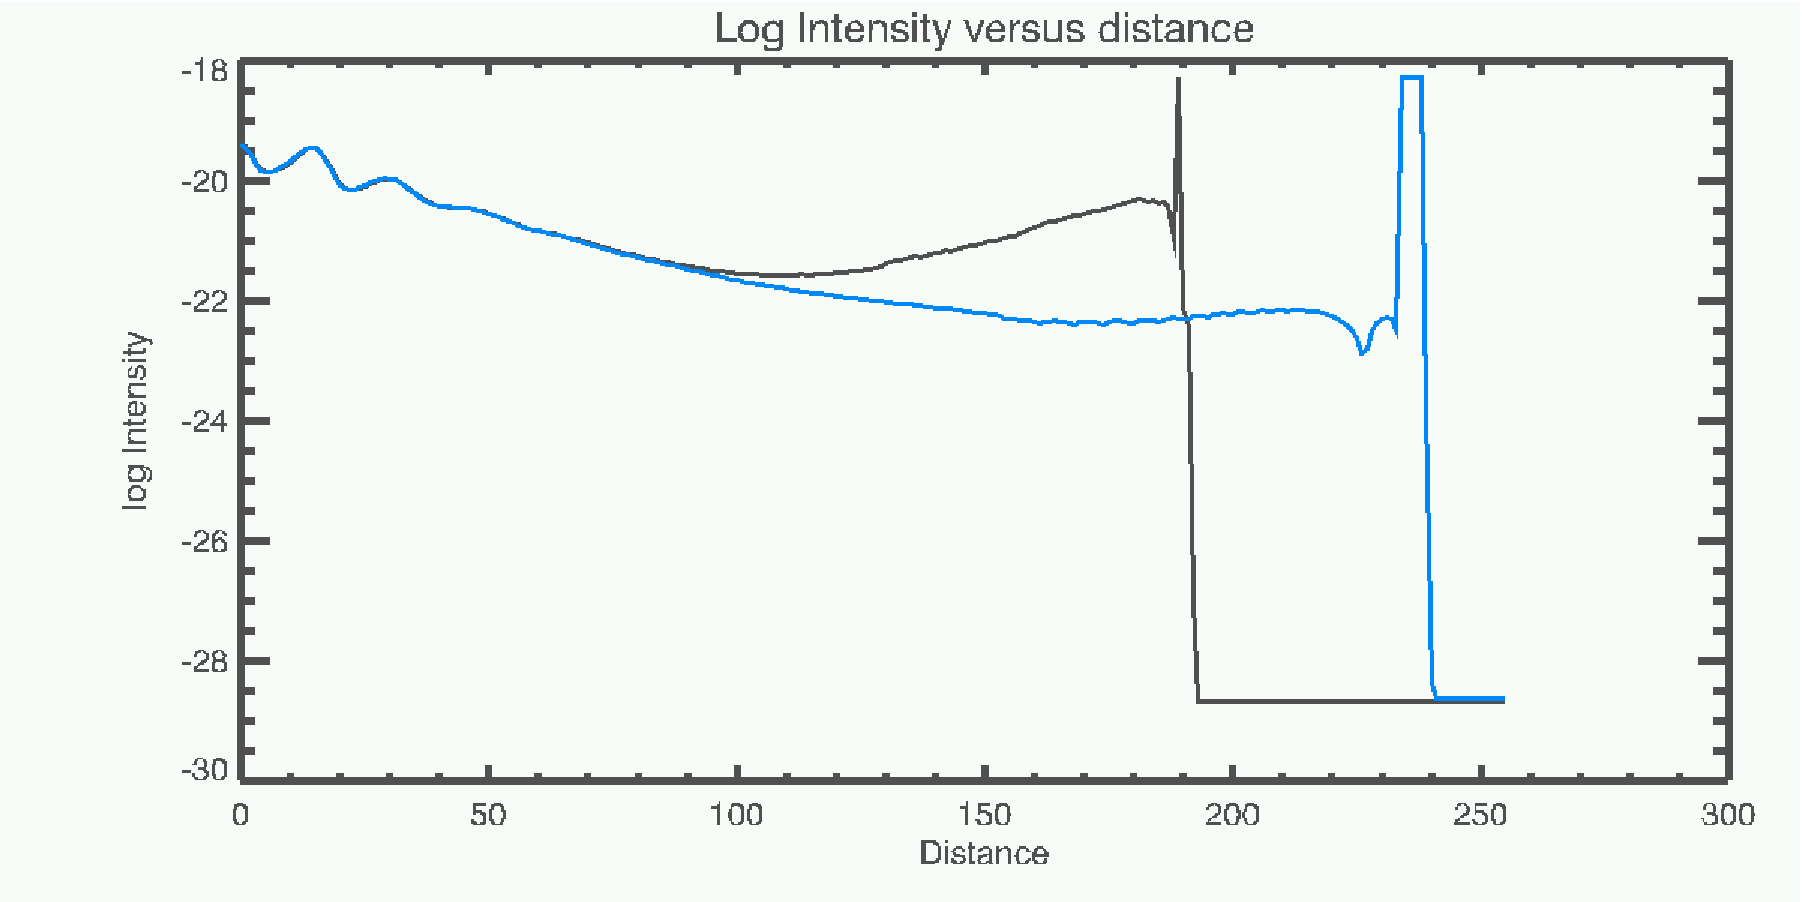
\includegraphics[width=9cm]{intensity_plot}
%\caption{
%Intensity of OII line emission along jet axis for evacuated and non-evacuated ambient medium.
%}
%\label{fig:43}       % Give a unique label
%\end{figure}


%\subsection{Case VI: Pulsed, non-adiabatic, three-dimensional jet in cavity}


%This case uses an evacuated cavity present for only half of the simulation.  The physical motivation is the idea of jet which has outpaced the preceding outburst. There should be a greater presence of cooling instabilities after the cavity has ended.  This serves as a counterexample to circulation model-type configuration, where the cavity starts to steepen far from the central source.  


\begin{figure*}[t]
\begin{center}
\begin{minipage}[t]{.48\linewidth}
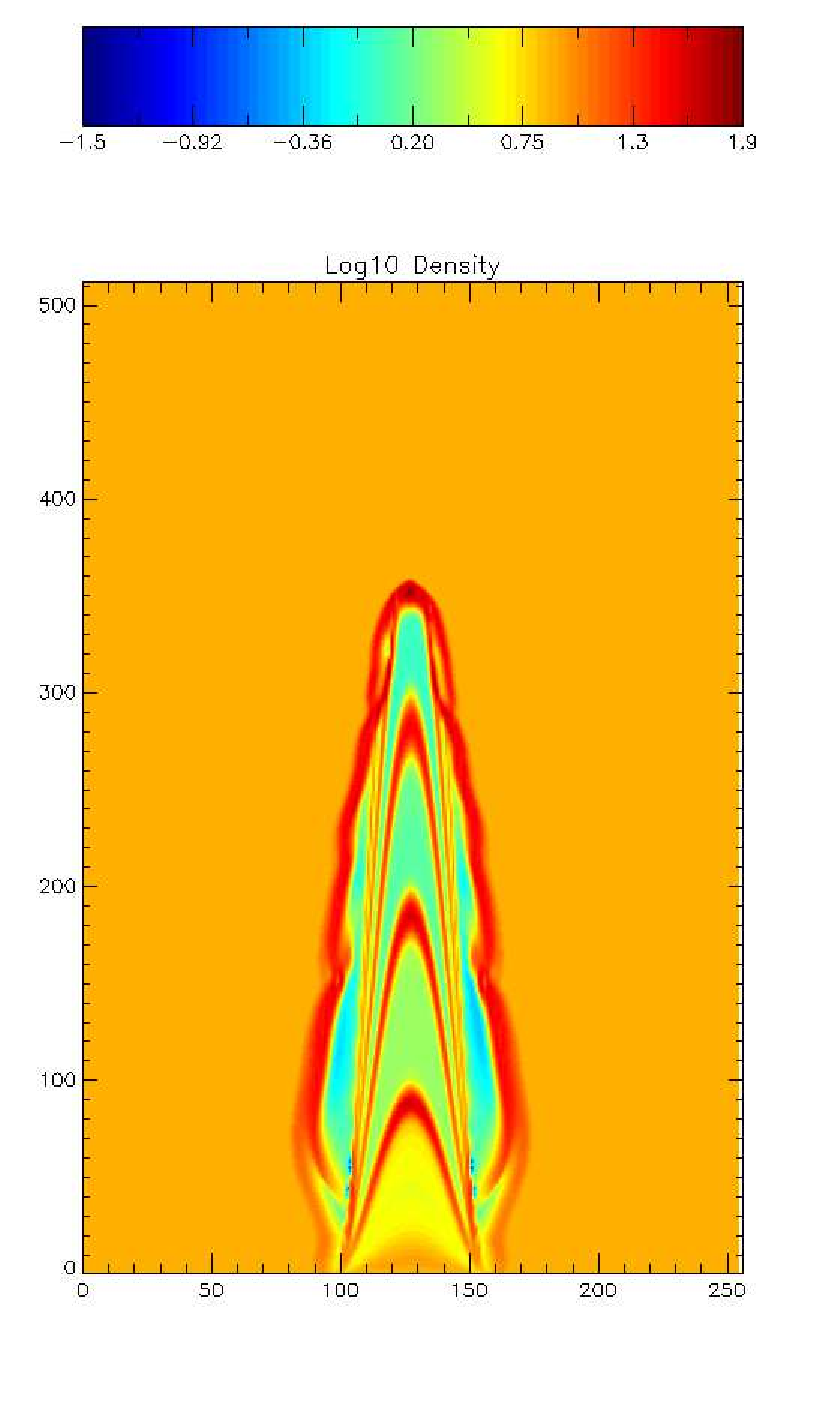
\includegraphics[width=8cm]{3dnogradden}
\end{minipage} \hfill
\begin{minipage}[t]{.48\linewidth}
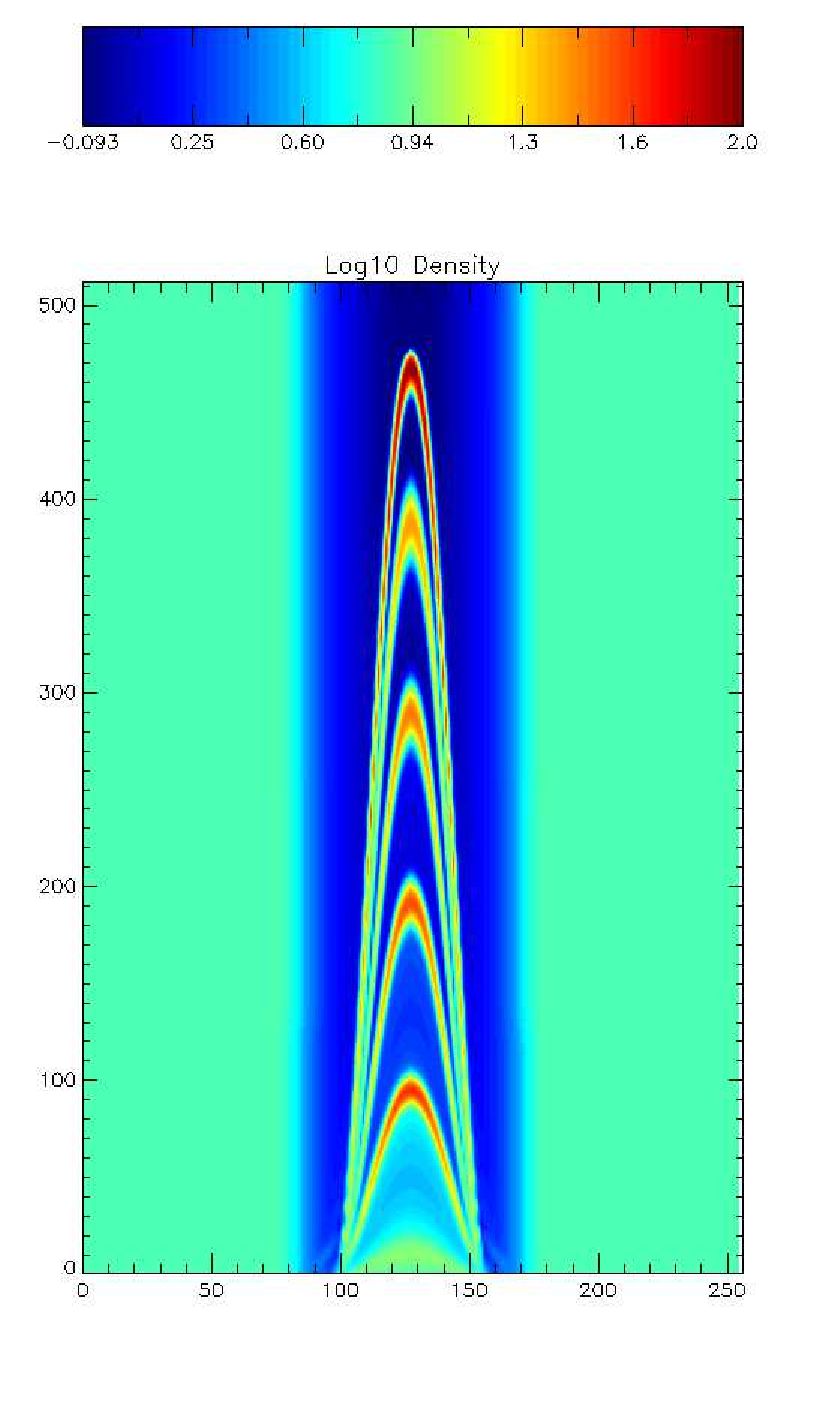
\includegraphics[width=8cm]{3dgradden}
\end{minipage}
\caption{ 
Left panel: Logscale density for 3d jet simulation without evacuated cavity 
at time t=588 years.
Right panel: Logscale density for 3d jet simulation in evacuated cavity 
at the same time.
}
\label{fig:3DDensity}       % Give a unique label
\end{center}
\end{figure*}

\begin{figure*}[t]
\begin{center}
\begin{minipage}[t]{.48\linewidth}
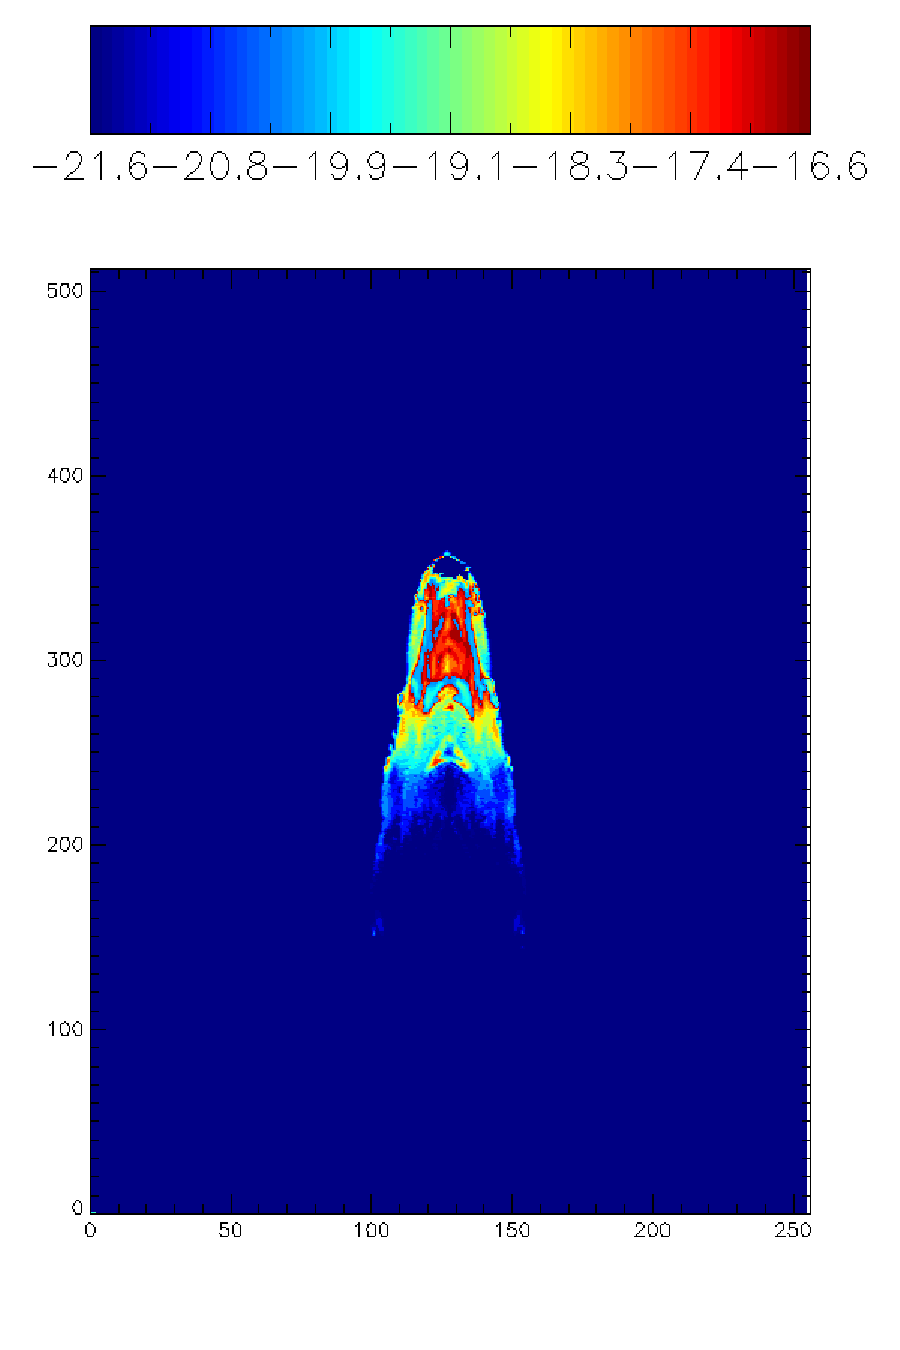
\includegraphics[width=8cm]{3dnograd}
\end{minipage} \hfill
\begin{minipage}[t]{.48\linewidth}
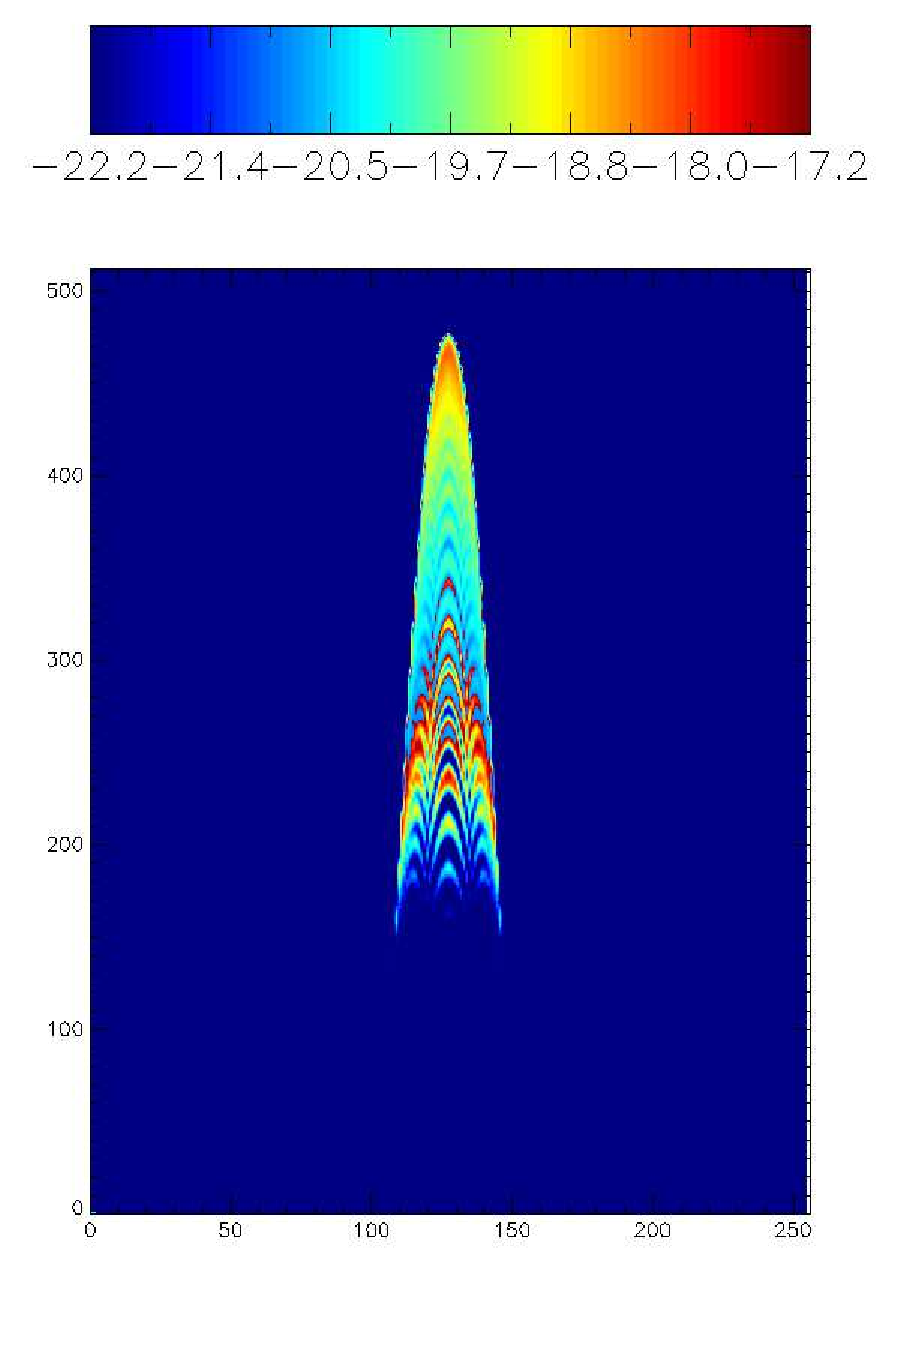
\includegraphics[width=8cm]{3dgrad}
\end{minipage}
\caption{ 
Left panel: Logscale H$\alpha$ line emission for 3d jet simulation without evacuated cavity 
Right panel: Logscale H$\alpha$ line emission for 3d jet simulation in evacuated cavity 
}
\label{fig:3DEmission}       % Give a unique label
\end{center}
\end{figure*}


%\begin{figure*}[t]
%\begin{center}
%\begin{minipage}[t]{.48\linewidth}
%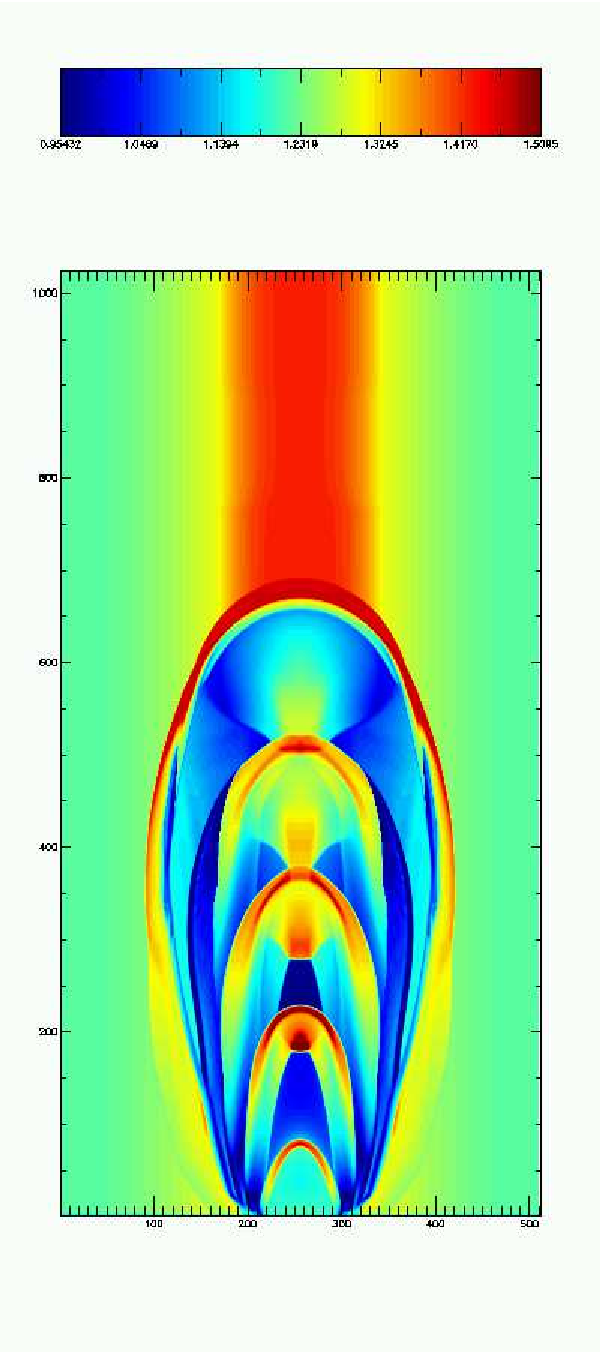
\includegraphics[angle=270,width=8cm]{g1a}
%\end{minipage} \hfill
%\begin{minipage}[t]{.48\linewidth}
%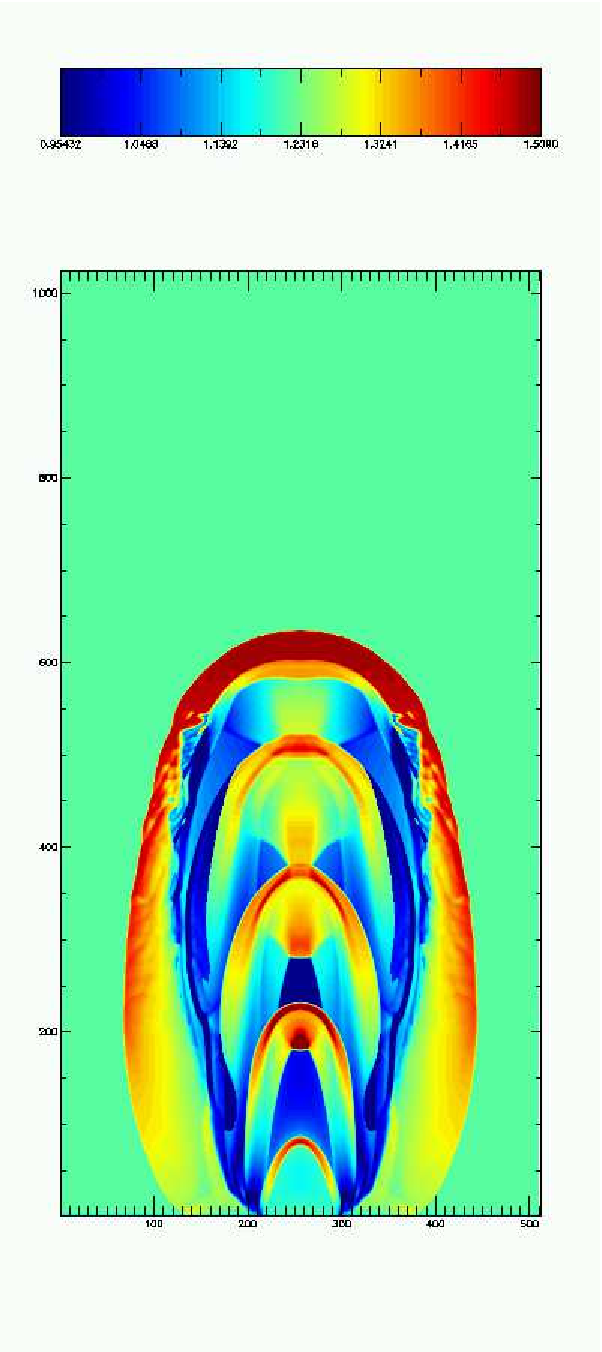
\includegraphics[angle=270,width=8cm]{g1b}
%\end{minipage}
%\caption{
%Sutherland and Dopita atomic emission map for 2d evacuated cavity jet integrated along line-of-sight.  This is not the emission from any specific line - but the entirety of instantaneous cooling at the indicated time.
%In each example the jet is propagated into the ambient medium.
%Left panel: results for cases with density gradients at time t=244 years.
%Right panel: results for cases without density gradients at time t=488 years.
%\label{fig:20}}
%\end{center}
%\end{figure*}


%\subsection{Emission Maps} 

%In order to be able to compare the simulations with observed phenomena it is necessary to convert the three-dimensional data images to maps of the intensity of the emission from the jets.
%Emission maps have been produced using
%Sutherland and Dopita atomic emission (Figure \ref{fig:20}) and integrating along line-of-sight.  This is not the emission from any specific line - but the entirety of instantaneous cooling at the indicated time.  H$\alpha$, SII, NII and OII line emission maps are produced.

\section{Discussion} 

\subsection{The effects of collimation and acceleration}

In the adiabatic cases, both Case I and Case II, there is extremely strong recollimation of the jet by the environment.
However in the overdense case, the dense bullets quickly overrun the evacuated cavity so the morphology is really only affected near the leading part of the jet.
In the underdense case the same argument applies.
However, including radiative cooling, (Case II and IV) the collimation is not so pronounced and the development of instabilities is hindered by the cavity.
This may be due to a combination of the pressure gradient compressing the jet towards the axis and the fact that the jet travels more quickly, so the instabilities have less time to develop and are more elongated when they do develop.

%Strong collimation is evident.
%The jet beam width is 50\% reduced.
%The FWHM
%The parameter space study shows
%The 3D model shows

%\subsection{The effects of acceleration}

%Strong acceleration is a natural consequence of the model.
%The parameter space study shows
%The 3D model shows

\subsection{Observational signatures of the circulation model}

%Observational signatures of the accretion model are strong recollimation far out and strong acceleration.
There are three possible main observational signatures of evacuated cavities.
The actual jet recollimation is quite gradual and would require high-resolution imagery over long distances for confirmation.
The acceleration by the cavity is also not a promising observational signature, as it require monitoring the jet over a long time period.
The decrease in radiative cooling losses may make the jet harder to observe when it enters a cavity.
%The dearth of cooling instabilities provides a more interesting line of thought.  The head of the jet is usually the most morphologically irregular HH knot, because it meets the ambient medium first and doesn't have a path carved out for it.  

%Need to look further out in the outflow for signs of the shocks and instabilities which typify this recollimation.
%Need to measure the densities.
%Need to check the velocities.

%Further work statistical studies of jets and outflows.

\subsection{Prehistory of jets}
The effects of collimation and acceleration 
caused by the evacuated cavity in the ambient medium are shown for both 2.5D (see Figure \ref{fig:flash:cool_pulse})  and 3D (see Figure \ref{fig:3DDensity}).
%In Figure \ref{fig:51} the distance by which the environmentally collimated jet has outpaced the standard case is particularly evident.

\section{Conclusions}


% have presented the theory of jet recollimation and performed some numerical simulations to show the effects of collimation and acceleration on the jet structure.

% have also produced some emission maps for comparison with observed highly collimated jets.

\begin{itemize}
\item Strong recollimation is demonstrated for parameters appropriate to Class I protostellar jets.
\item Strong acceleration is obtained far from the protostar for parameters appropriate to Class I protostellar jets.
\item A dependence of acceleration and collimation on $\eta$ and density decrement, $\delta$ is established.
\item New possible methods for detecting the observational signatures of the circulation model are proposed.
\item For the investigated parameters, the density and pressure gradient appears to compress the cocoon and the density reduction in the path of the bow shock decreases the amount of vortex shedding and mixing, resulting in a less morphologically rich cocoon environment.

\end{itemize}

\begin{table}
\begin{center}
\begin{tabular}{l c c c}
\hline
       & Density Decrement  &Aspect Ratio& Bow Shock Advance Speed\\
\hline
\hline
 Case I &  1& 2.5    &  240 km/s\\
  &  10&  5    &  340 km/s\\
\hline
 Case II &1&   2.5    &  73 km/s\\
  &  10& 6    &  156 km/s\\
\hline
 Case III &1&   4.4   &  151 km/s\\
  &  10& 8   &  223 km/s\\
\hline
 Case IV &1&   4    & 136  km/s\\
  & 10&  7.1    &  223 km/s\\
\hline
 \end{tabular}
 \caption{Jet aspect ratios and bow shock advance speeds for cases I-IV}
\label{AspectRatiosandAdvanceSpeeds}
 \end{center}
 \end{table}
